\documentclass[conference]{IEEEtran}
\usepackage[utf8]{inputenc}
\usepackage{amsmath,amsfonts}
\usepackage{mathtools}
\usepackage{graphicx} 
\usepackage{cite}
\usepackage{hyperref}
\usepackage{float}
\usepackage{placeins}
\usepackage{gensymb}

\begin{document}

\title{Quadrature Down Converter \\ \Large Design, Simulations and Applications}

\author{
    \IEEEauthorblockN{
        Madhur Kankane\IEEEauthorrefmark{1}, 
        Het Asit Selarka\IEEEauthorrefmark{2}, 
        Siddhant Gudwani\IEEEauthorrefmark{3}
    }
    \IEEEauthorblockA{\IEEEauthorrefmark{1}ECE, IIIT Hyderabad, India\\
    Roll No: 2024102061\\
    Email: madhur.kankane@students.iiit.ac.in}
    \IEEEauthorblockA{\IEEEauthorrefmark{2}ECE, IIIT Hyderabad, India\\
    Roll No: 2024102031\\
    Email: het.selarka@students.iiit.ac.in}
    \IEEEauthorblockA{\IEEEauthorrefmark{3}ECE, IIIT Hyderabad, India\\
    Roll No: 2024102042\\
    Email: siddhant.gudwani@students.iiit.ac.in}
}


\maketitle

\begin{abstract}
This paper presents the design, simulation, and functional analysis of a quadrature down-converter. It begins with a brief overview of the purpose and applications of down-conversion, followed by a detailed breakdown of the system into its fundamental components. Each part is examined to highlight its role in the overall operation. The individual elements are then integrated into a complete circuit. Finally, the paper provides a comparative analysis of theoretical simulations and practical results, validating the effectiveness and accuracy of the proposed design for each individual components as well the practical challenges faced while integrating the final down converter.
\end{abstract}

\begin{IEEEkeywords}
quadrature, oscillator, down conversion, mixer,
filter, image rejection, modulation, switch, in-phase, quadrature phase
\end{IEEEkeywords}

\section{Introduction}
Modern wireless communication systems require efficient
frequency translation techniques to process high-frequency
signals. Quadrature downconversion is a widely used approach
in receiver front-ends, particularly in applications such as
Bluetooth, Wi-Fi, and other RF systems. It enables the ex-
traction of in-phase (I) and quadrature-phase (Q) components
of a signal, which are essential for digital modulation and
demodulation techniques.

\begin{figure}[H]
\centering
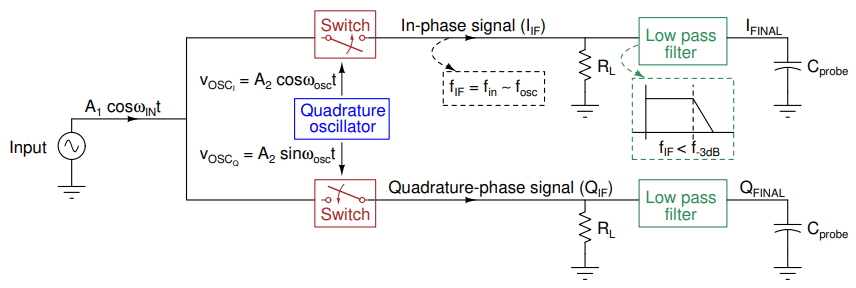
\includegraphics[scale=0.45]{intro.png}
\caption{Block diagram for a Quadrature Down Converter}
\end{figure}

As shown above, the input signal $v_{in} = A_1 \cos \omega_{in} t$ is 
mixed with $v_{OSC_I} = A_2 \cos \omega_{OSC} t$ and 
$v_{OSC_Q} = A_2 \sin \omega_{OSC} t$ 
to produce in-phase and quadrature-phase signals respectively, 
with a phase difference of 90\degree. Mixing of these two signals 
is the same as their product, which may be simplified to:

\begin{align*}
v_{IF_I} &= \frac{A_1 A_2}{2} \left( \cos(\omega_{in} - \omega_{OSC})t + \cos(\omega_{in} + \omega_{OSC})t \right) \\
v_{IF_Q} &= \frac{A_1 A_2}{2} \left( \sin(\omega_{in} + \omega_{OSC})t - \sin(\omega_{in} - \omega_{OSC})t \right)
\end{align*}

These signals are fed to a low-pass filter so that only the difference frequency is obtained at $I_{FINAL}$ and $Q_{FINAL}$, which is quite low, and the very high sum frequency is filtered out.


In this project, we design and simulate a quadrature down-
converter using analog building blocks such as a quadrature os-
cillator, mixer (switch), and low-pass filter. All circuit modules
are implemented and analyzed using LTSpice. The objective is
to demonstrate frequency downconversion of a high-frequency
input signal into its intermediate frequency (IF) components
while preserving phase information.

The simulation-based approach enables performance evalu-
ation of individual blocks and the complete system, focusing
on aspects such as waveform behavior, frequency spectra, and
I/Q signal isolation.

\section{Significance and Application of Quadrature Down Converter}
Quadrature down-conversion plays a vital role in modern communication systems due to its ability to process complex modulated signals efficiently. The following points highlight its significance:

\subsection{Information Recovery}

Modern digital modulation schemes such as QAM and PSK encode information in both amplitude and phase. To accurately recover this information, the receiver must:

\begin{itemize}
    \item Preserve both amplitude and phase relationships,
    \item Process positive and negative frequency components independently,
    \item Maintain orthogonality between signal components.
\end{itemize}

The in-phase and quadrature (I-Q) architecture achieves this by utilizing two parallel signal paths with a 90° phase difference.

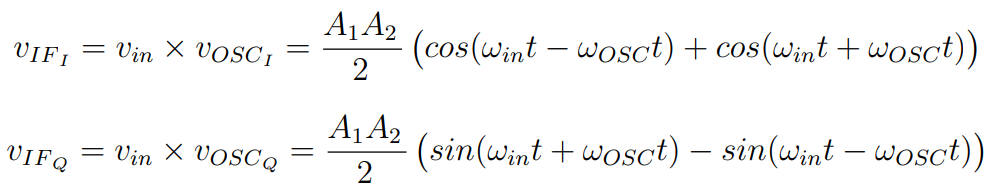
\includegraphics[scale=0.34]{info_recovery.png}

\subsection{Image Rejection}

Image rejection is a critical application of quadrature processing. In conventional heterodyne receivers, an image frequency at \( 2f_{LO} - f_{RF} \) can interfere with the desired signal. Quadrature architectures eliminate this image through internal signal processing, rather than relying on bulky external filters, thus reducing component count and enabling higher levels of integration.

\begin{figure}[H]
\centering
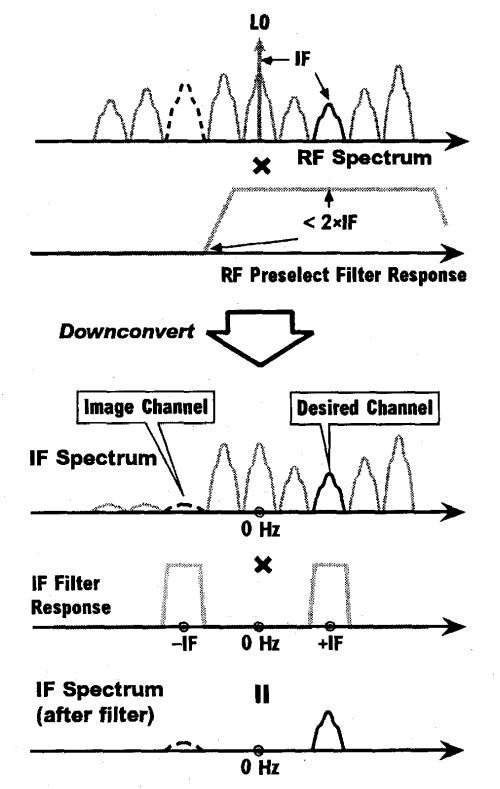
\includegraphics[scale=0.62]{image_rej1.png}
\caption{Image rejection in quadrature processing}
\end{figure}

\begin{figure}[h]
\centering
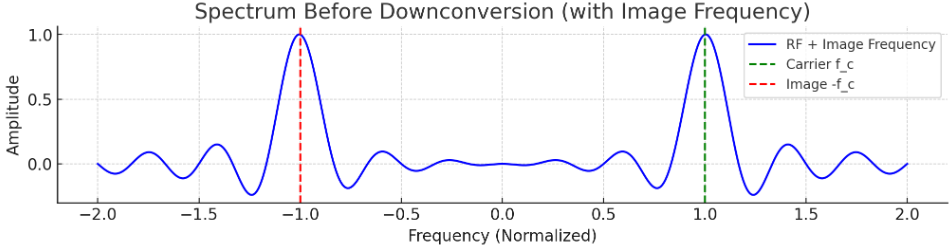
\includegraphics[scale=0.34]{image_rej2.png}
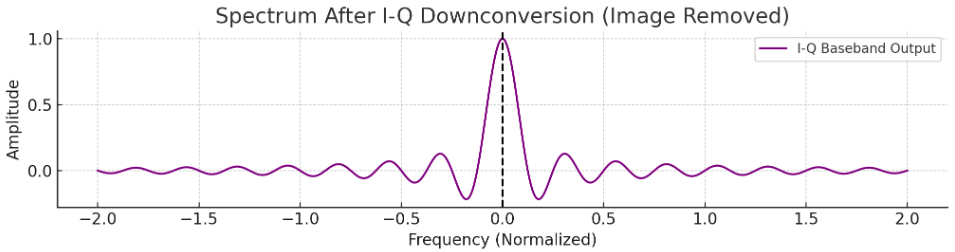
\includegraphics[scale=0.34]{image_rej3.png}
\caption{Orthogonal Demodulation Image term folds into Orthogonal phase and cancels}
\end{figure}

\subsection{Spectral Efficiency}

Quadrature processing enhances spectral efficiency by transmitting information on both I and Q channels. This effectively doubles the data throughput within the same bandwidth compared to single-channel systems. Such efficiency is essential in modern wireless systems, where spectrum is both scarce and expensive.

\subsection{Hardware Simplification and Complex Modulation Support}

Quadrature processing simplifies hardware design by:

\begin{itemize}
    \item Replacing bulky intermediate-frequency (IF) and image-reject filters with integrated analog or digital signal processing,
    \item Supporting advanced modulation schemes like 64-QAM through independent modulation of I and Q components,
    \item Enabling software-defined operation compatible with multiple communication standards.
\end{itemize}

\section{QUADRATURE OSCILLATOR}

\begin{figure}[H]
\centering
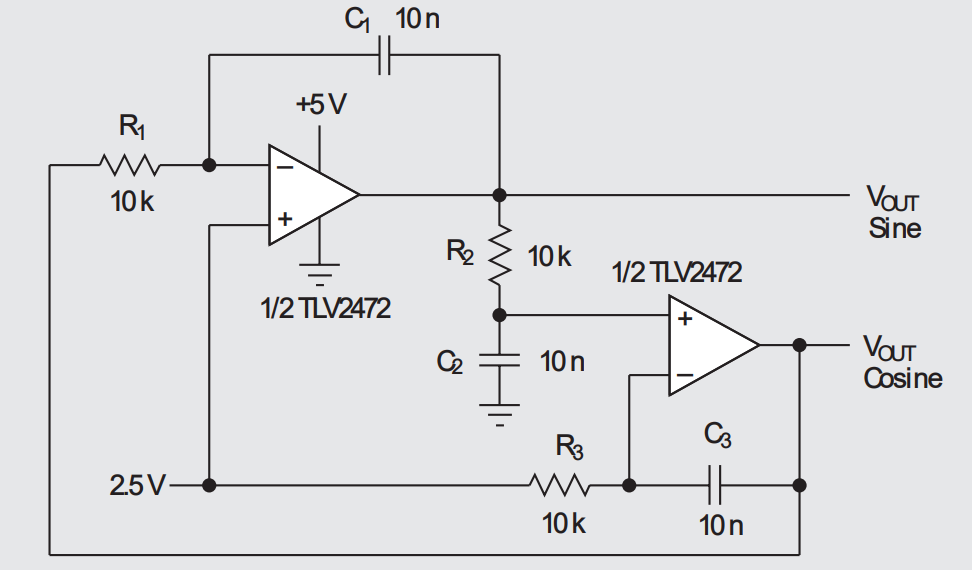
\includegraphics[scale=0.4]{quad_scematic.png}
\caption{Schematic of Quadrature oscillator}
\end{figure}

A quadrature oscillator is designed to generate two sinusoidal signals with a 90° phase difference. The topology employed utilizes two operational amplifiers (op-amps), each contributing to the generation of these phase-shifted waveforms. The circuit, illustrated in Fig. 2, can be understood by analyzing it in two stages.

In the first stage, the initial op-amp functions as an integrator, with a capacitor providing negative feedback from the output to the input. When a sinusoidal input—such as a cosine wave—is applied, the output of this op-amp becomes a sine wave, effectively achieving a 90° phase shift. This output is then passed through an RC filter to suppress high-frequency components.

In the second stage, the filtered signal serves as the input to the second op-amp, which also operates as an integrator. Consequently, if a sine wave is input to this stage, the output becomes a cosine wave—reconstructing the original input. Through this configuration, the circuit continuously regenerates two sinusoidal signals that are 90° out of phase, thus realizing quadrature oscillation.
\begin{figure}[h]
\centering
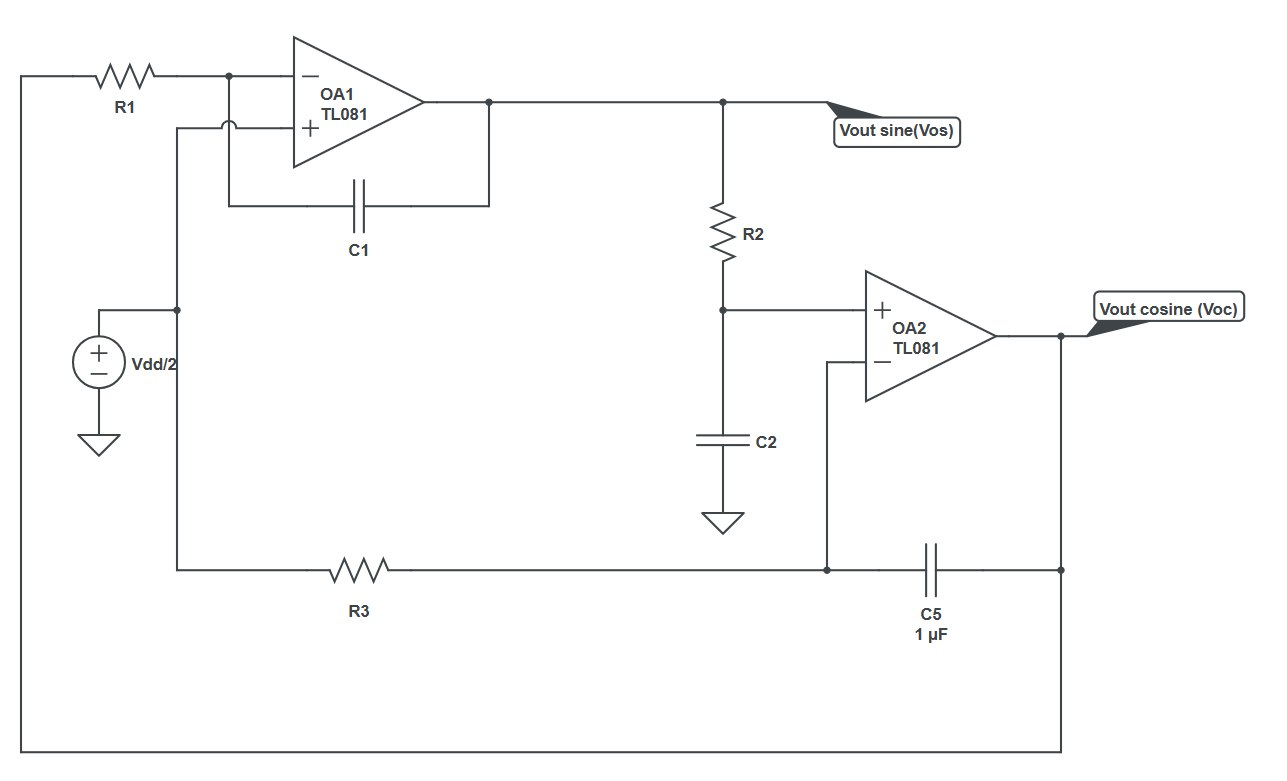
\includegraphics[scale=0.33]{Quad_topo.jpeg}
\caption{Topology of Quadrature oscillator}
\end{figure}

\section*{Calculations}
Traversing from $V_{O_S}$ to $V_{+_2}$ ; $V_{+_2}$ to $V_{O_C}$ ; $V_{O_C}$ to $V_{O_S}$ loop:-
\begin{itemize}
    \item $V_{O_S} \rightarrow V_{+_2}$
    \\ As we can see, it is a simple voltage divider:
    $$\Rightarrow  V_{+_2} = \frac{\frac{1}{C_2S}}{R_2+\frac{1}{C_2S}} V_{O_S}$$
    \begin{align}
    \Rightarrow\Aboxed{V_{+_2}=\frac{1}{1+R_2C_2S}V_{O_S}}   
    \end{align}

    \item $V_{+_2} \rightarrow V_{O_C}$
    \begin{figure}[h]
    \centering
    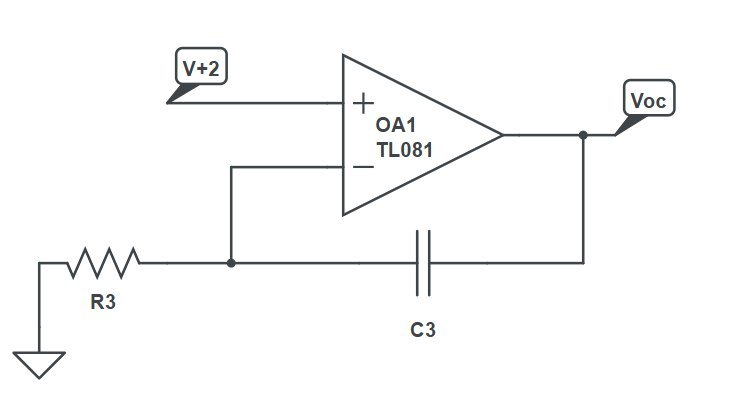
\includegraphics[scale=0.37]{non_inverting.jpeg}
    \caption{Non-Inverting Amplifier}
    \end{figure}
    $$V_{O_C} = \left( 1+ \frac{\frac{1}{C_3S}}{R_3} \right) V_{+_2}$$
    \begin{align}
    \Rightarrow\Aboxed {V_{O_C} = \frac{1 + R_3C_3S}{R_3C_3S}V_{+_2}}
    \end{align}

    \item $V_{O_C} \rightarrow V_{O_S}$
    \begin{figure}[h]
    \centering
    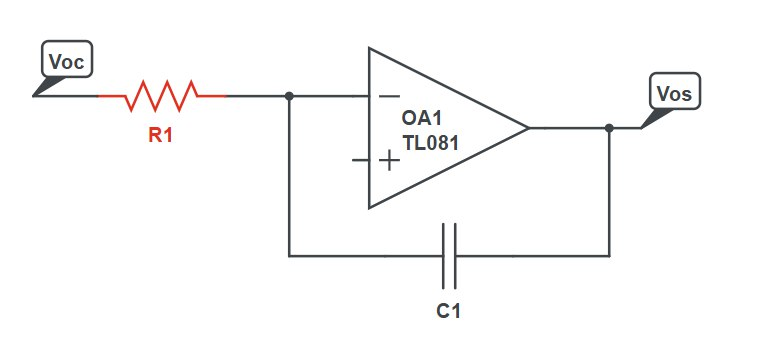
\includegraphics[scale=0.4]{inverting.jpeg}
    \caption{Inverting Amplifier}
    \end{figure}
    $$V_{O_S} = \left( -\frac{\frac{1}{C_1S}}{R_1} \right) V_{O_C}$$
    \begin{align}
    \Rightarrow\Aboxed {V_{O_S} = -\frac{1}{R_1C_1S}V_{O_C}}
    \end{align}

    The loop gain of the system should be 1 for a stable oscillation.
    $$\Rightarrow (1)\times(2)\times(3)=1$$
    $$-\frac{1}{R_1C_1S}\times\frac{1+R_3C_3S}{R_3C_3S}\times\frac{1}{1+R_2C_2S}=1$$
    Substituting $S=j\omega$, we get
    $$-\frac{1}{R_1C_1(j\omega)}\times\frac{1+R_3C_3(j\omega)}{R_3C_3(j\omega)}\times\frac{1}{1+R_2C_2(j\omega)}=1$$
    For practical purposes let us design it such that
    \begin{align}
    \Rightarrow\Aboxed {R_1C_1=R_2C_2=R_3C_3}
    \end{align}
    $$\Rightarrow-\frac{1}{(RC)^2(j\omega_0)^2}=1$$
    $$\Rightarrow\omega_0=-\frac{1}{RC}$$
    \begin{align}
    \Rightarrow\Aboxed{f_{osc}=\frac{\omega_{osc}}{2\pi}=\frac{1}{2\pi RC}}   
    \end{align}
    $$\Rightarrow RC=\frac{1}{2\pi f_{osc}}$$
    $\rightarrow$ We are required to obtain $f_{osc}= 100KHz$
    $$\Rightarrow RC=\frac{1}{2\pi\times100\times10^3} \approx 1.59\times10^{-6}$$
     $\rightarrow$ For our circuit let's take the value of 
     \begin{align}
     \Aboxed {R=5K\Omega}
     \end{align}
     $$\Rightarrow C= 0.318nF$$
     \begin{align}
     \Aboxed {C\approx0.32nF}
     \end{align}
     $\rightarrow V_{DD}/V_{SS}$ depends upon the Op-Amp model selection. In our case, we have used UA741. So we will take $V_{DD} = 5V$ and $V_{SS}=2.5V$
    
\end{itemize}

\subsection{Simulations}
\begin{figure}[H]
\centering
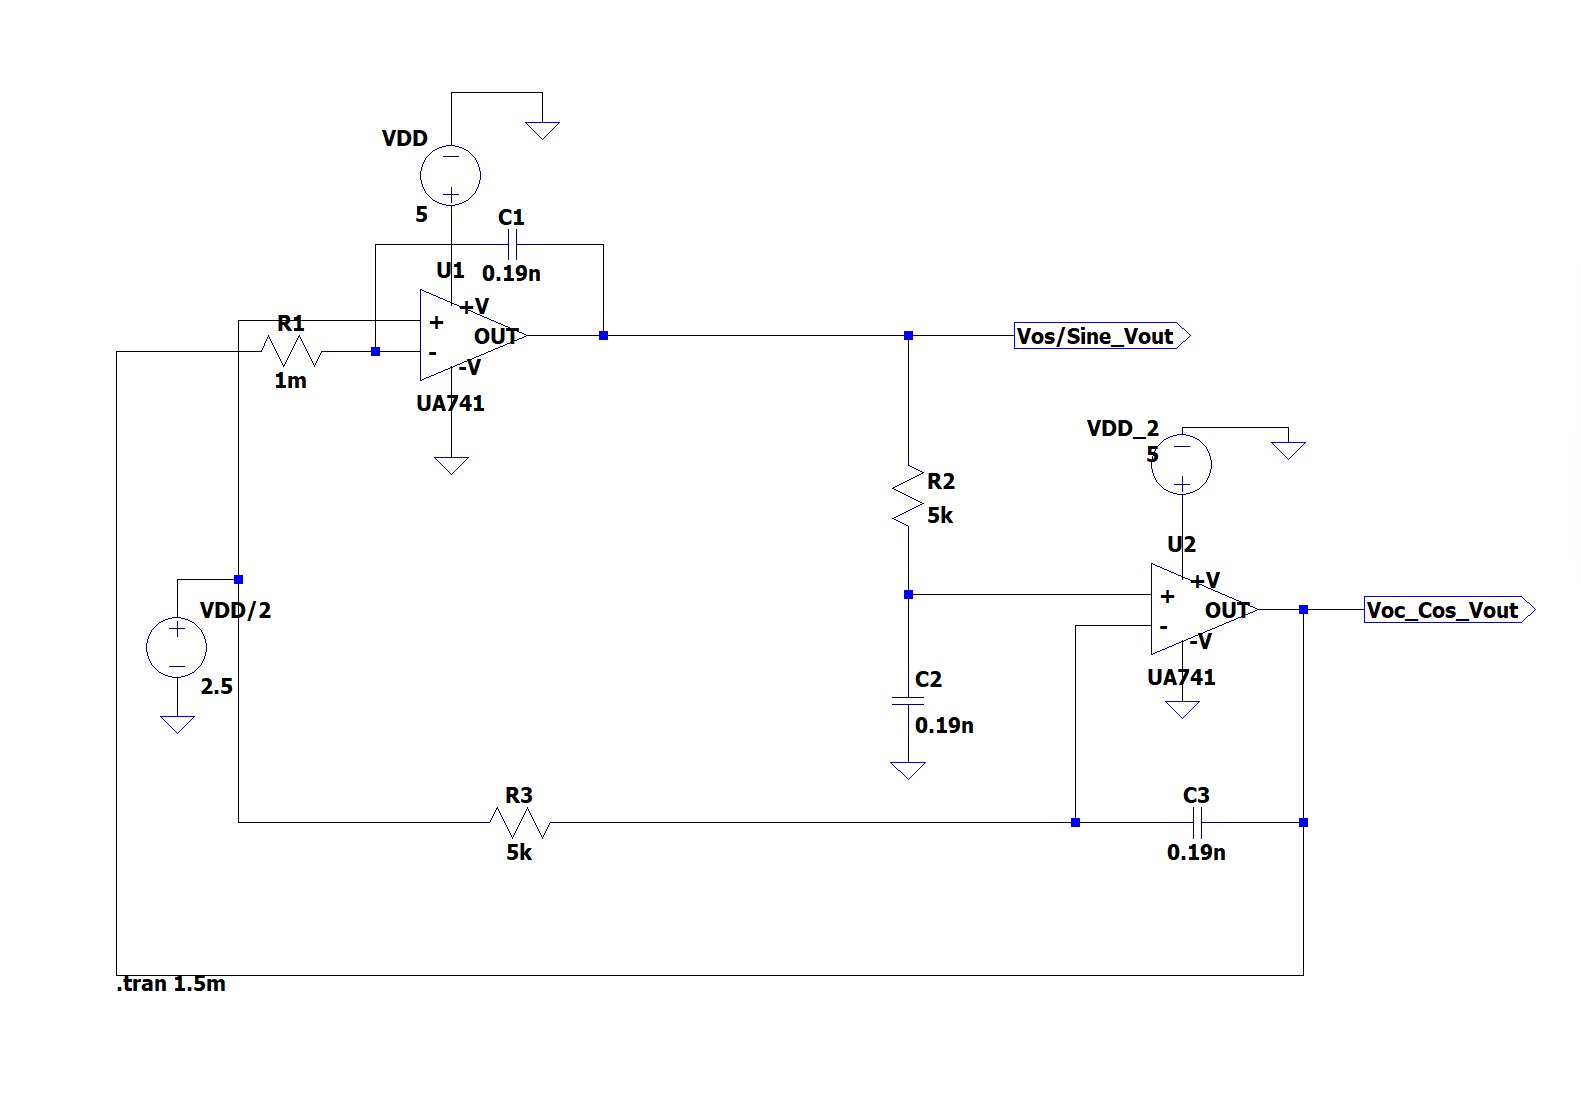
\includegraphics[scale=0.25]{quad_LT.jpeg}
\caption{Realizing oscillator on LTSPICE.}
\end{figure}

\begin{figure}[H]
\centering
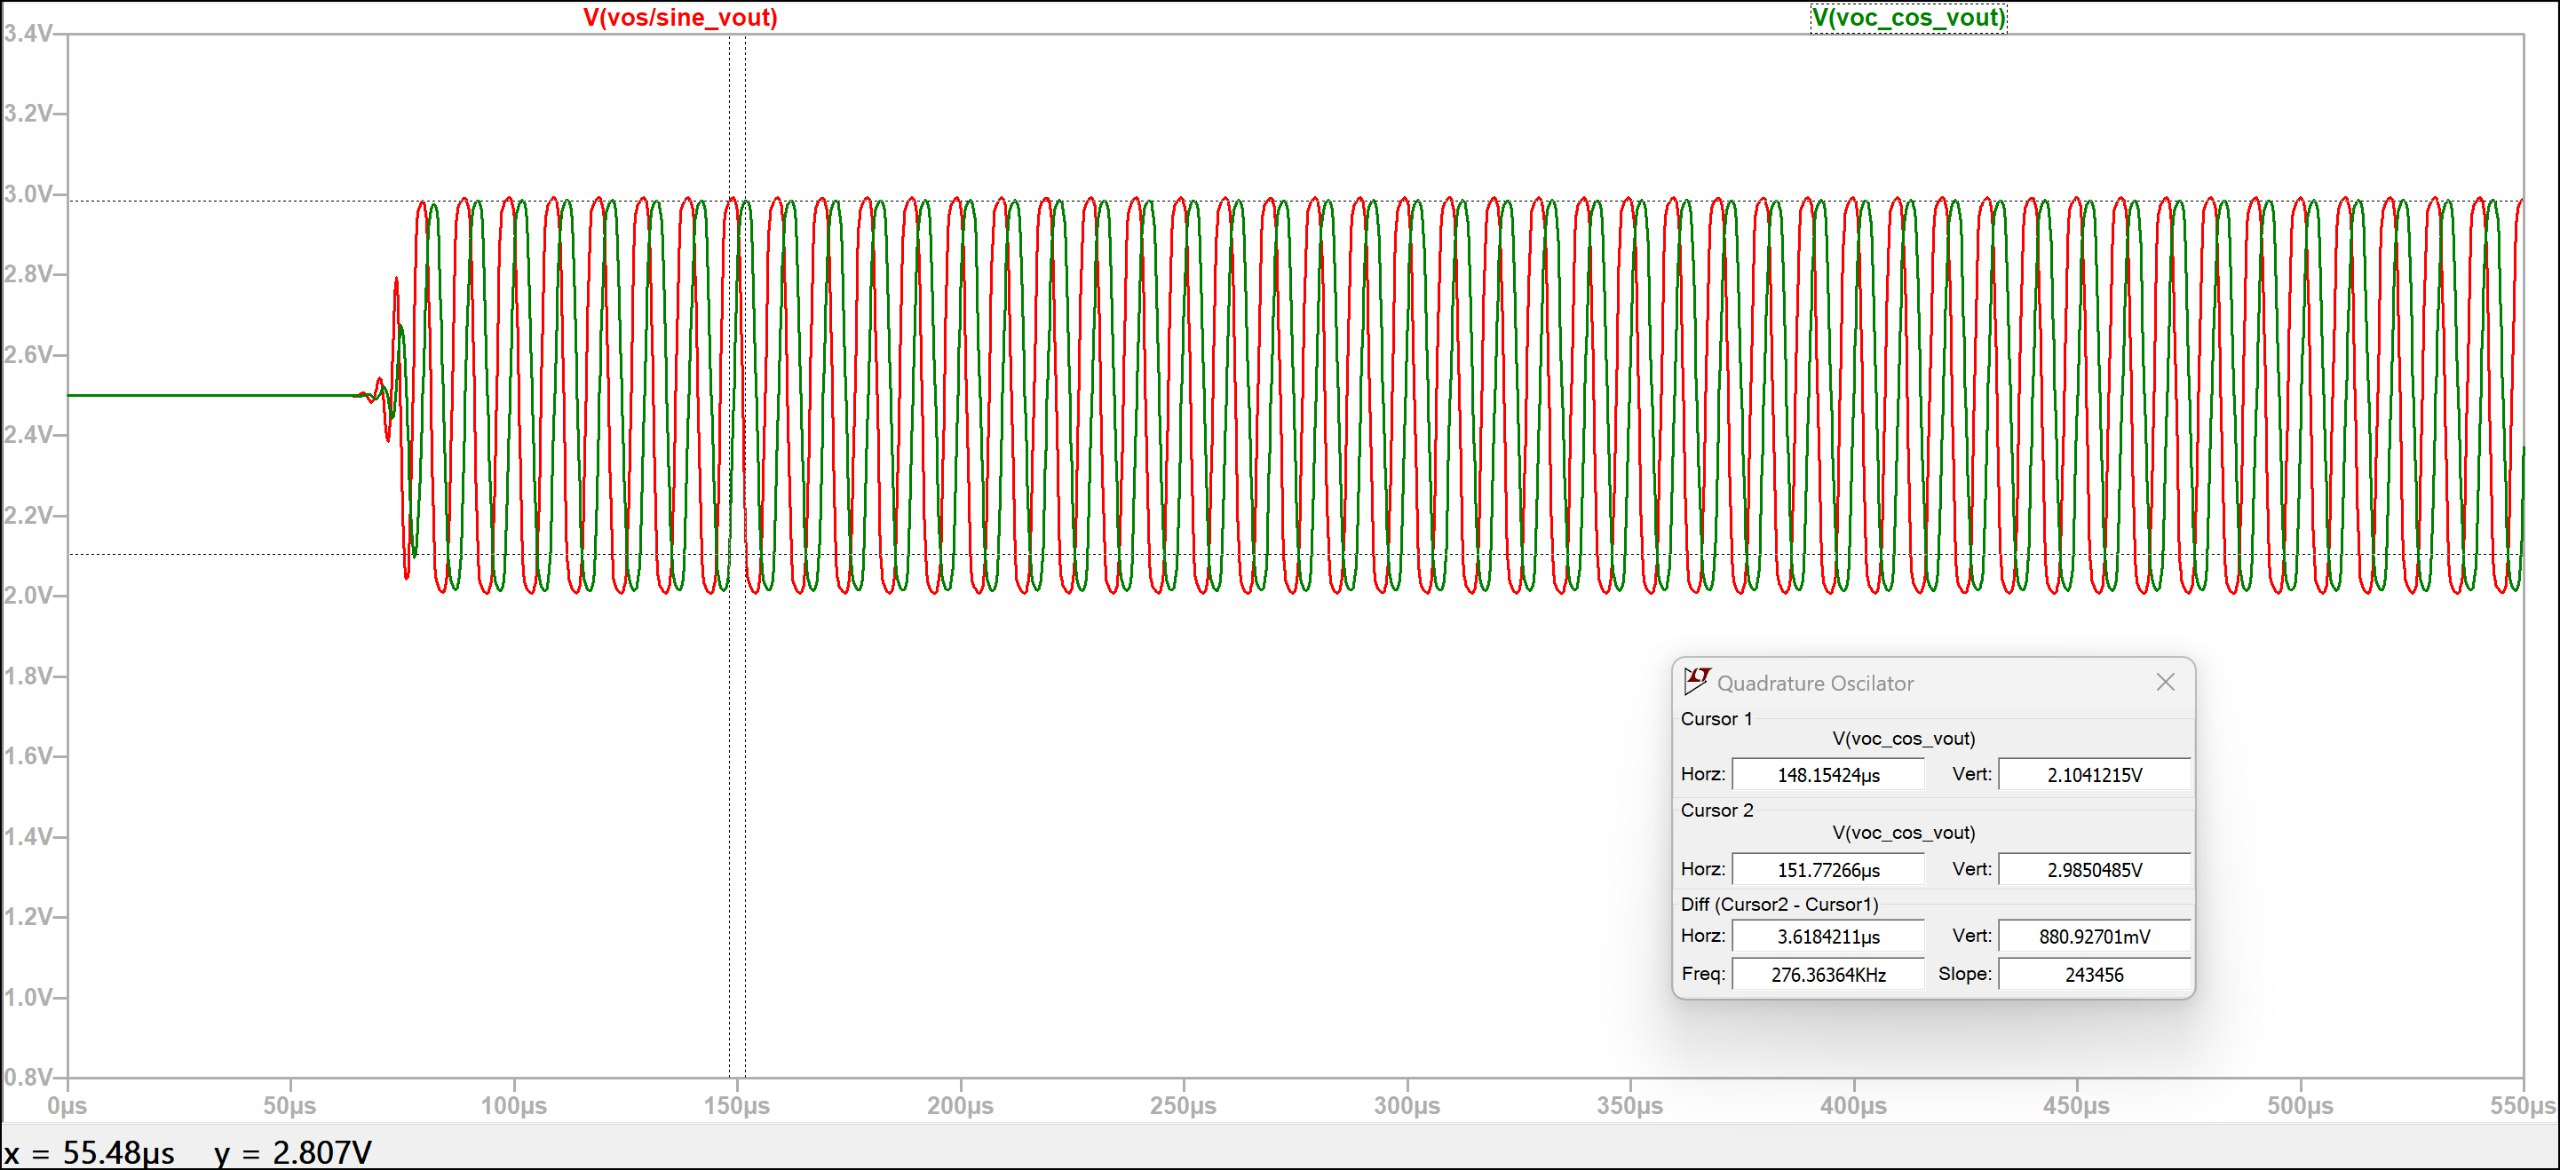
\includegraphics[scale=0.1]{quad_tran.jpeg}
\caption{}
\end{figure}

\begin{figure}[H]
\centering
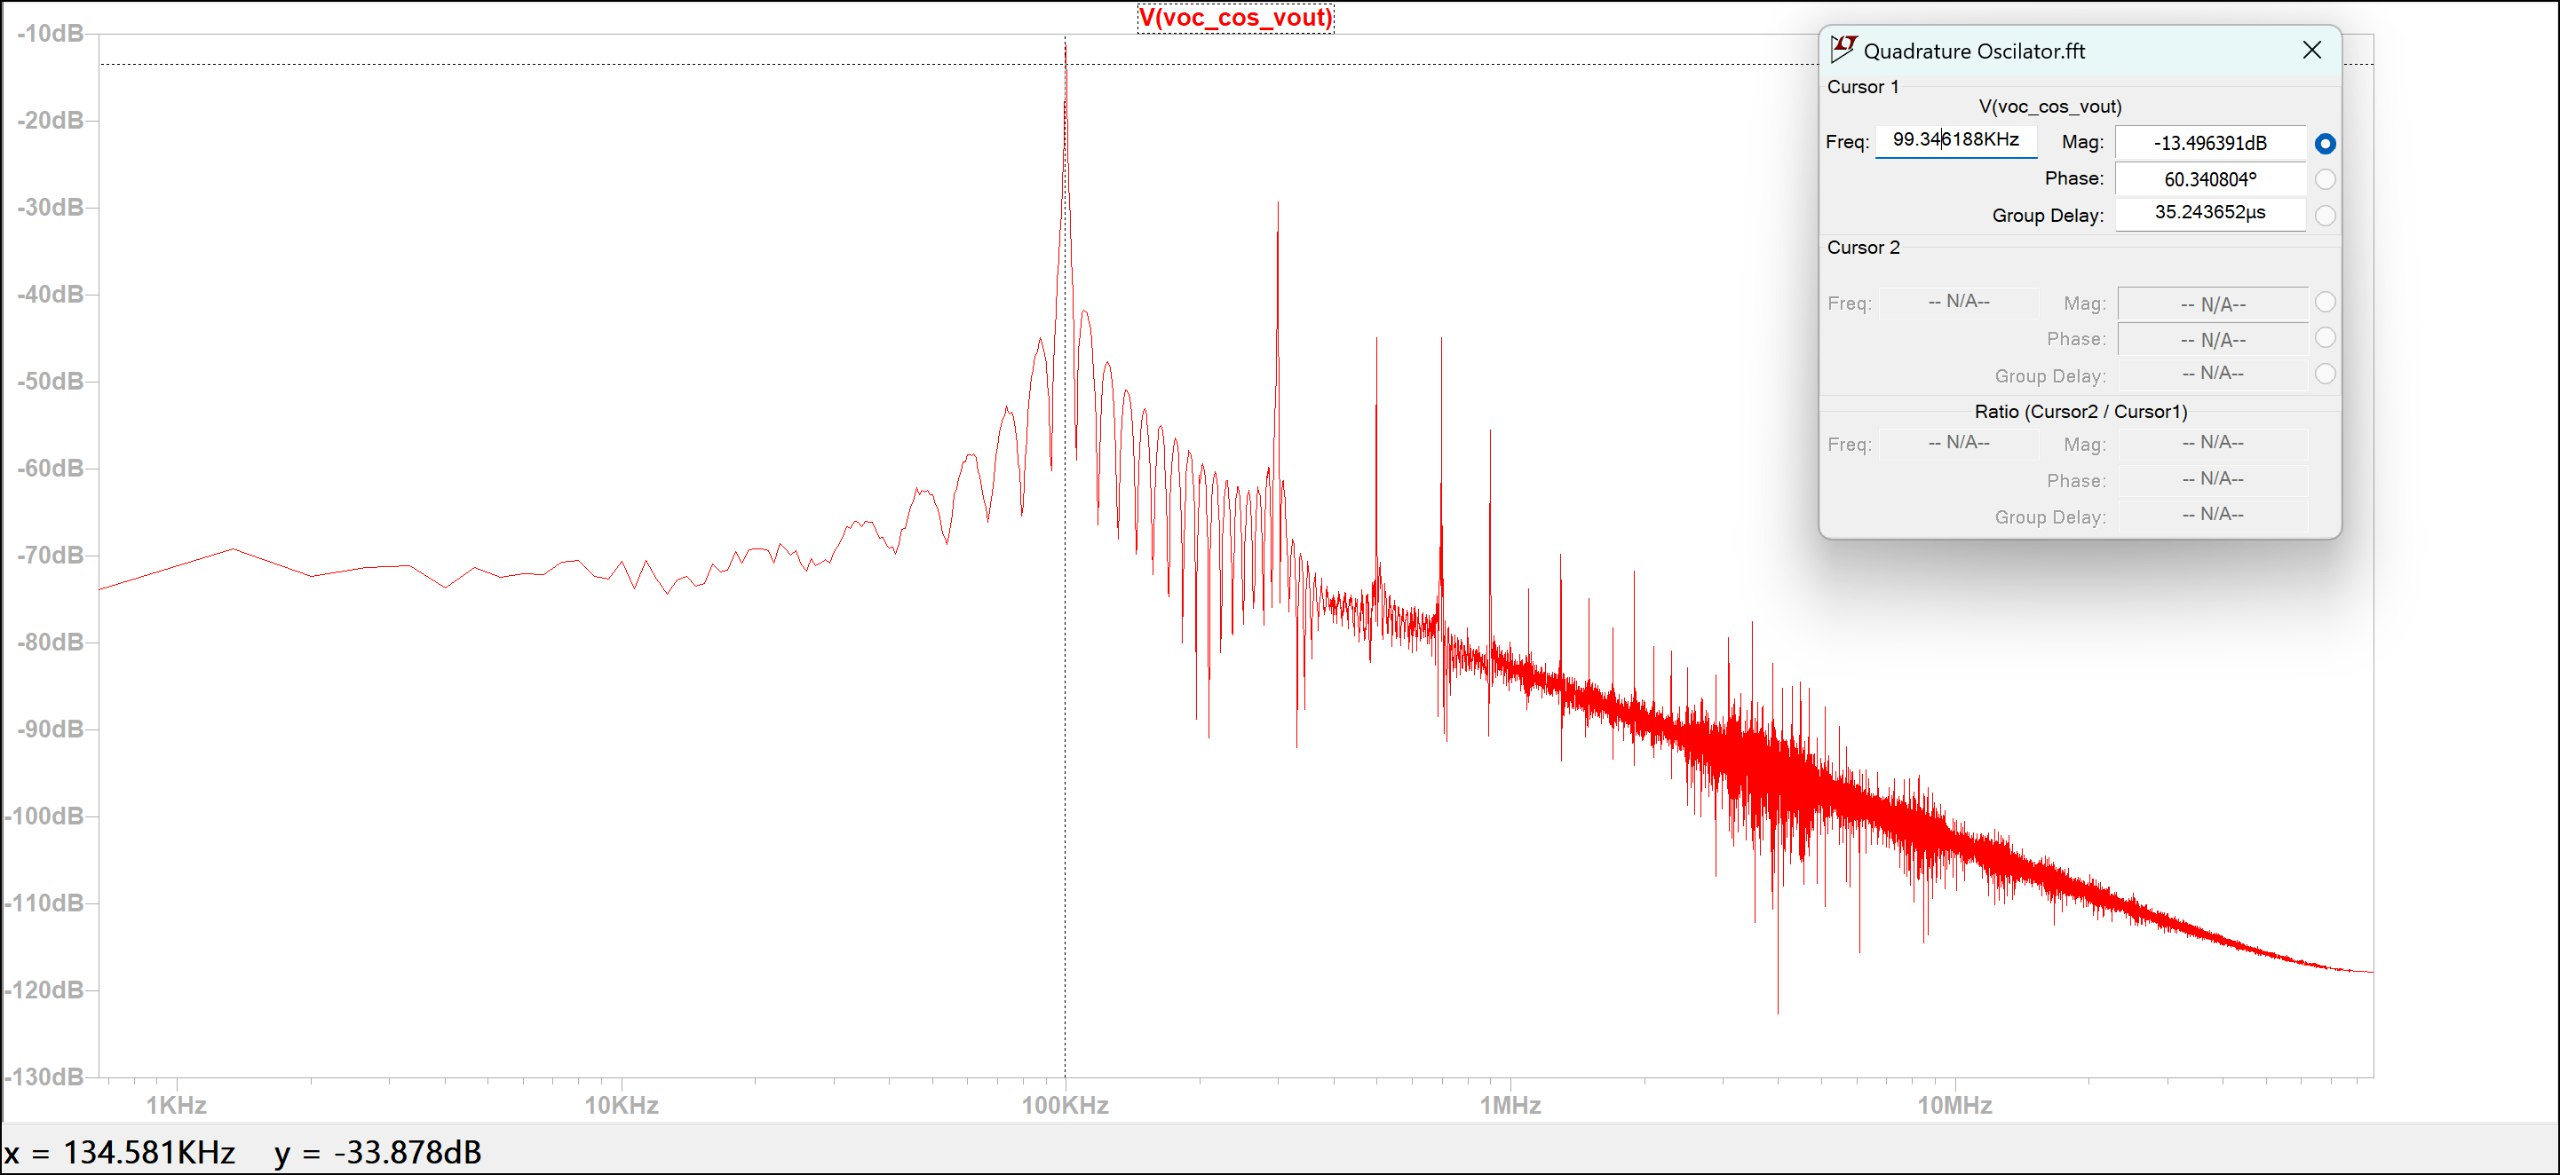
\includegraphics[scale=0.1]{quad_cos.jpeg}
\caption{FFT plot of Cosine wave which is output of our simulation}
\end{figure}

\begin{figure}[H]
\centering
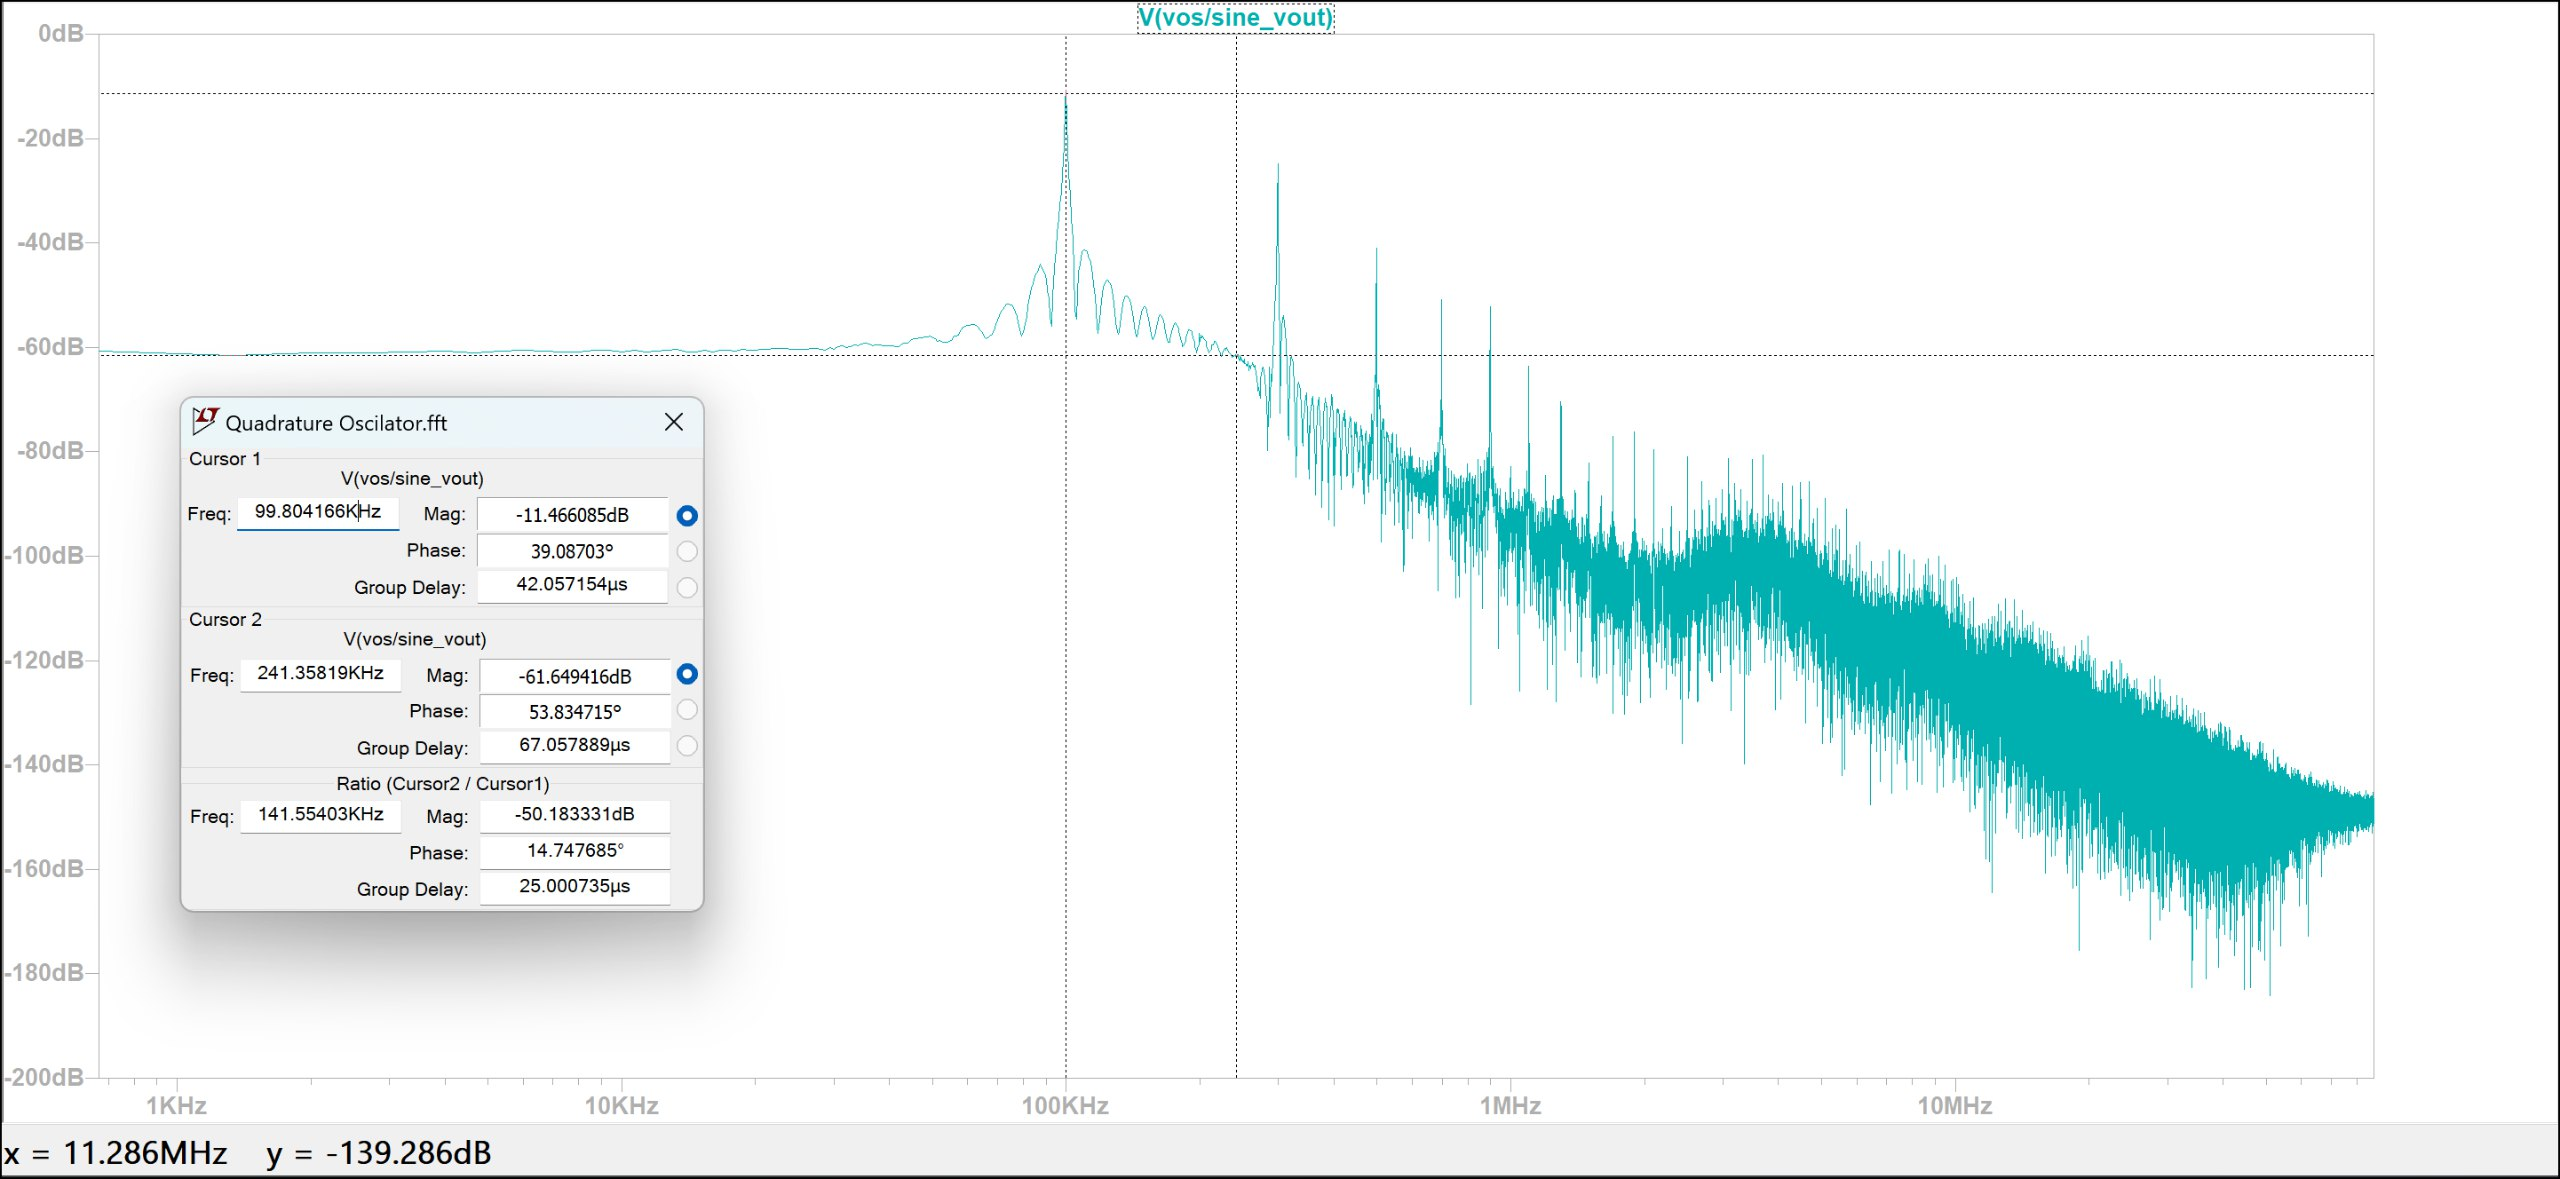
\includegraphics[scale=0.1]{quad_sin.jpeg}
\caption{ FFT plot of Sine wave which is output of our simulation}
\end{figure}

\begin{figure}[H]
\centering
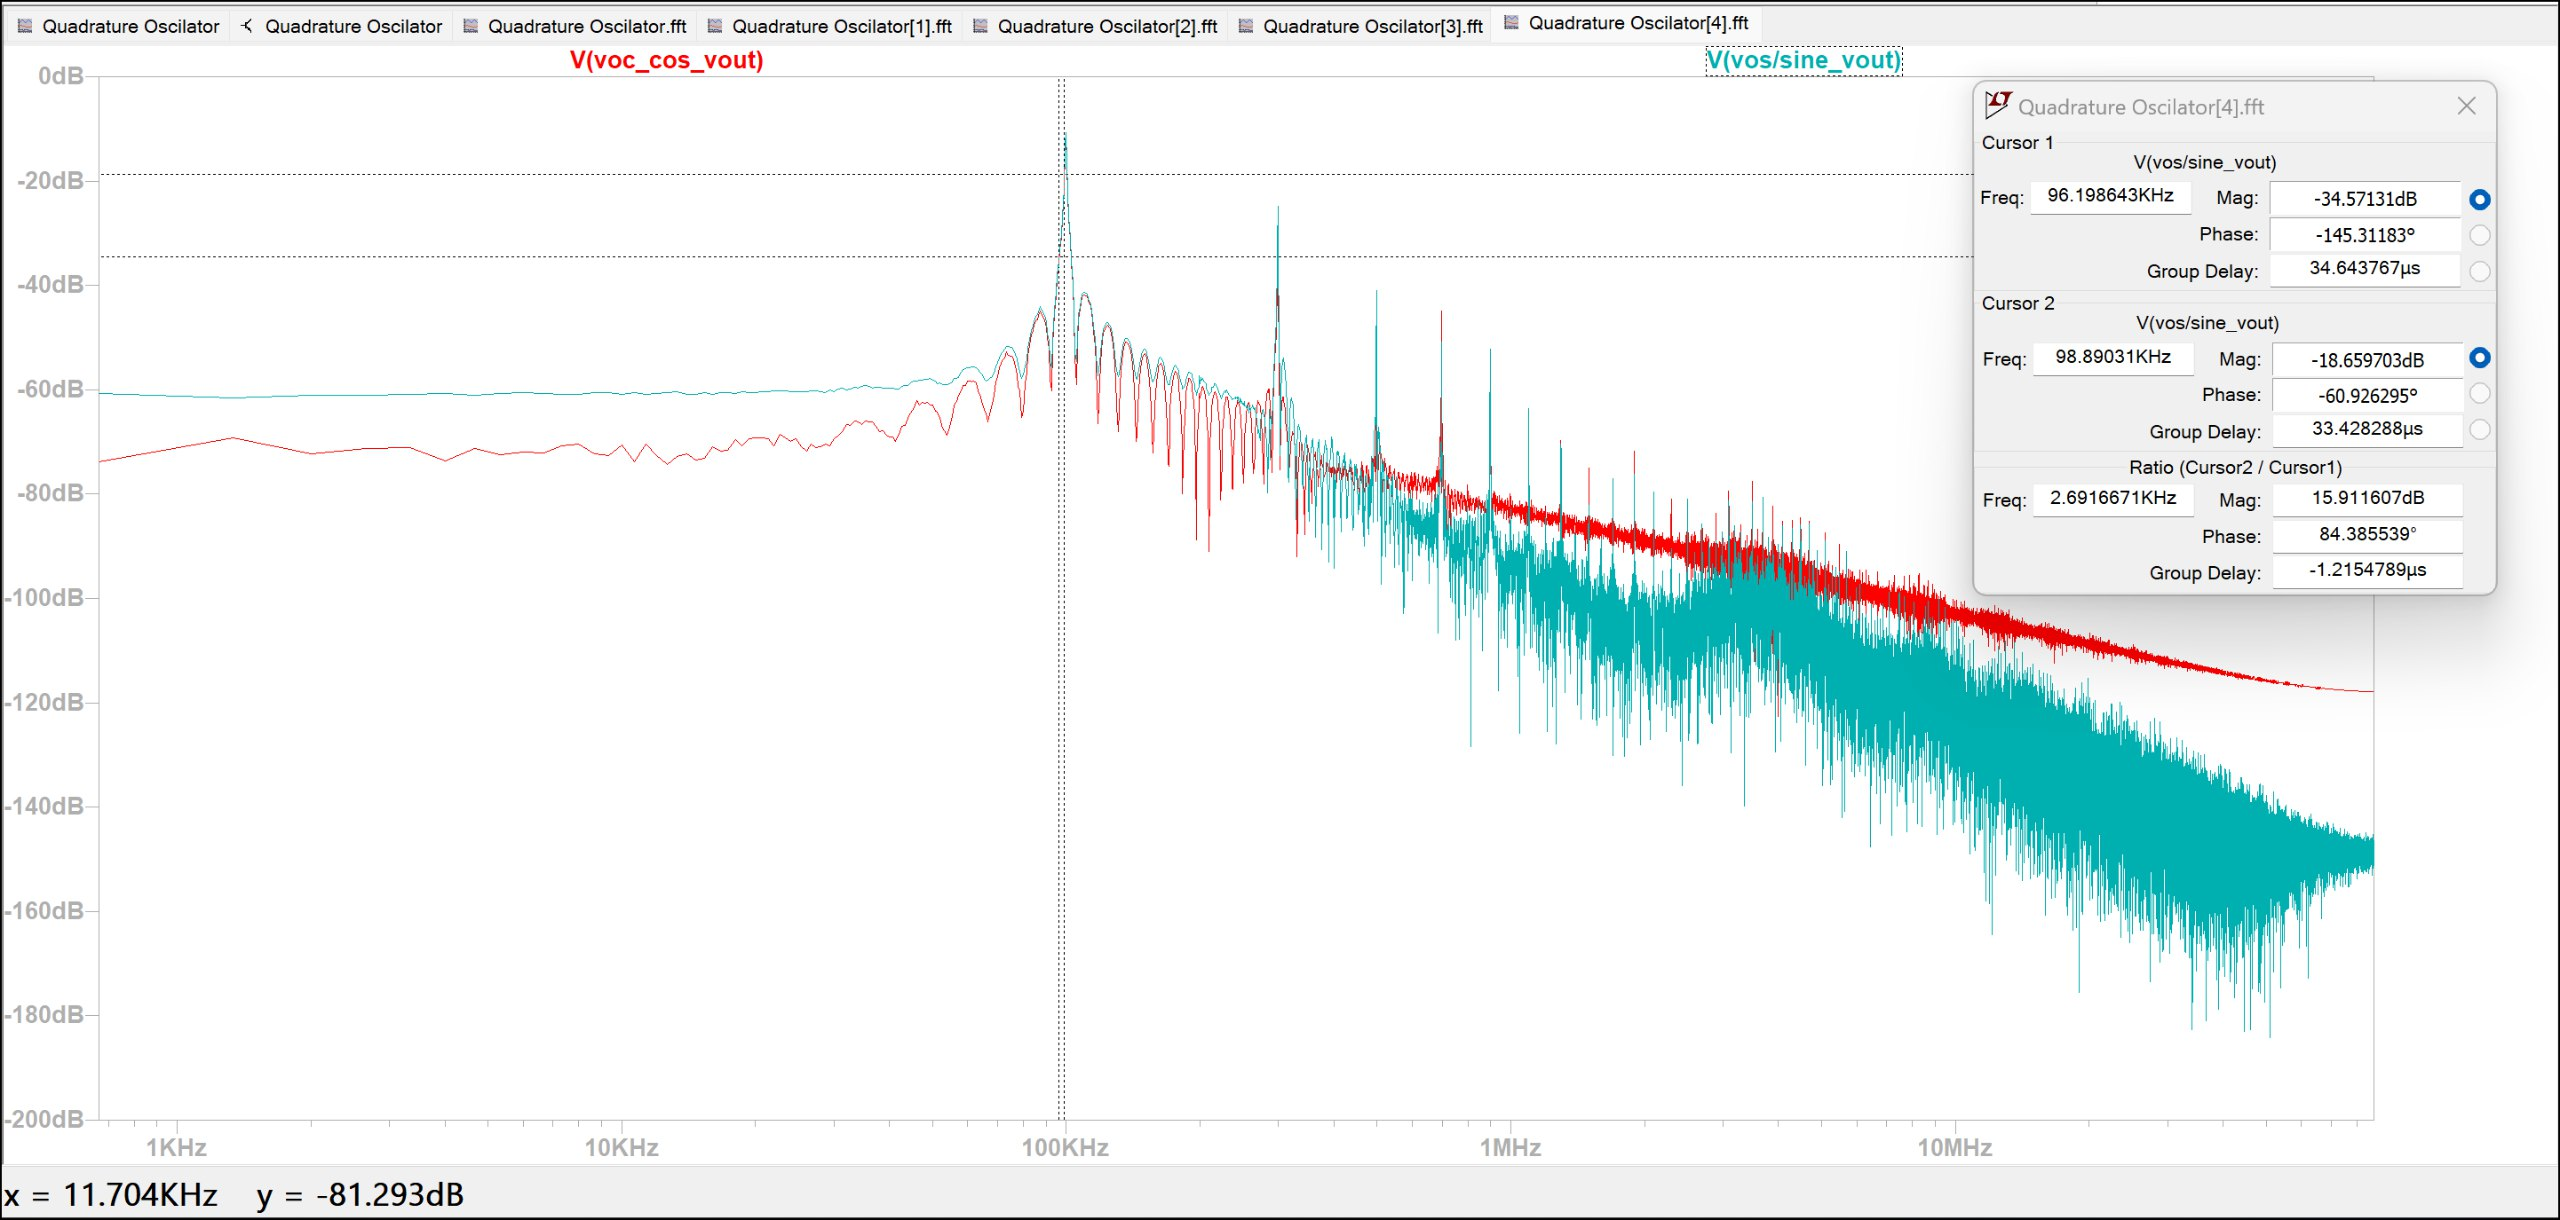
\includegraphics[scale=0.1]{quad_fft.jpeg}
\caption{ Combined FFT plot showing $90\degree$ phase difference}
\end{figure}

\section{Switch(Mixer) Design}
The primary goal of our project is to down-convert a high-frequency input signal to a lower output frequency. Specifically, Our aim is to extract the original message frequency from a modulated input signal that comprises both the carrier and the message frequencies. This is accomplished by generating a high-amplitude signal at the desired message frequency and filtering out all unwanted frequency components.

The core device used for this frequency translation is the mixer, which combines the message signal with a signal generated by a quadrature oscillator. The mixer effectively blends these two inputs to produce new frequency components, including the desired message frequency.

\begin{figure}[H]
\centering
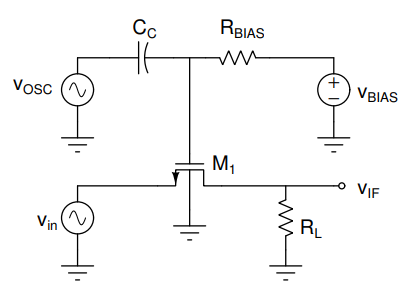
\includegraphics[scale=1]{mixer_cir.png}
\caption{Switch(Mixer) circuit}
\end{figure}

A mixer/switch functions as a signal multiplier; it multiplies two input signals. A basic mixer configuration consists of a MOSFET, a coupling capacitor, a bias and a load resistor, and a DC supply as bias voltage.

In our design, the oscillator frequency ($V_{OSC}$) is set equal to the carrier frequency, while the bias voltage($V_{BIAS}$)  is chosen close to the MOSFET’s threshold voltage. From the perspective of the oscillator, the circuit behaves as a high-pass filter—allowing AC components to pass while blocking DC. Conversely, from the bias voltage side, it acts as a low-pass filter—blocking AC and passing only DC.

As a result, the gate of the MOSFET receives a composite signal: an AC component from the oscillator superimposed on a DC offset provided by ($V_{BIAS}$) when ($V_{OSC}>0$), the MOSFET operates in the linear (on)  region and when ($V_{OSC}<0$), it switches off (cutoff region). This alternating on-off behavior essentially mimics a switching action at the oscillator frequency.

\subsection{(Intuitive) Working of Mixer}
\begin{itemize}
    \item From the circuit, the voltage at the gate terminal is observed to be:
    \[
    V_{GS} = V_{OSC} + V_{BIAS} = V_{OSC} + V_T
    \]
    
    \item For the NMOS transistor to conduct, it must be in the linear region, which requires:
    \[
    V_{GS} \geq V_T
    \]
    Conversely, if \( V_{GS} < V_T \), the MOSFET operates in the cutoff region.
    
    \item During the positive half-cycles of the oscillator signal:
    \[
    V_{OSC} + V_T \geq V_T \Rightarrow V_{GS} \geq V_T
    \]
    This implies the MOSFET is on, allowing the signal at the source terminal to pass through to the drain terminal, where the mixer output is taken.
    
    \item During the negative half-cycles of the oscillator signal, by similar reasoning, \( V_{GS} < V_T \). Hence, the MOSFET turns off, and the channel between source and drain is cut off.
    
    \item Since the oscillator frequency is high, the signal rapidly oscillates between positive and negative values, effectively switching the MOSFET on and off. This switching behavior produces a square-wave-like modulation that mixes with the input signal at the output of the mixer.
\end{itemize}

\subsection{Design,Simulation and Results}
\begin{figure}[H]
\centering
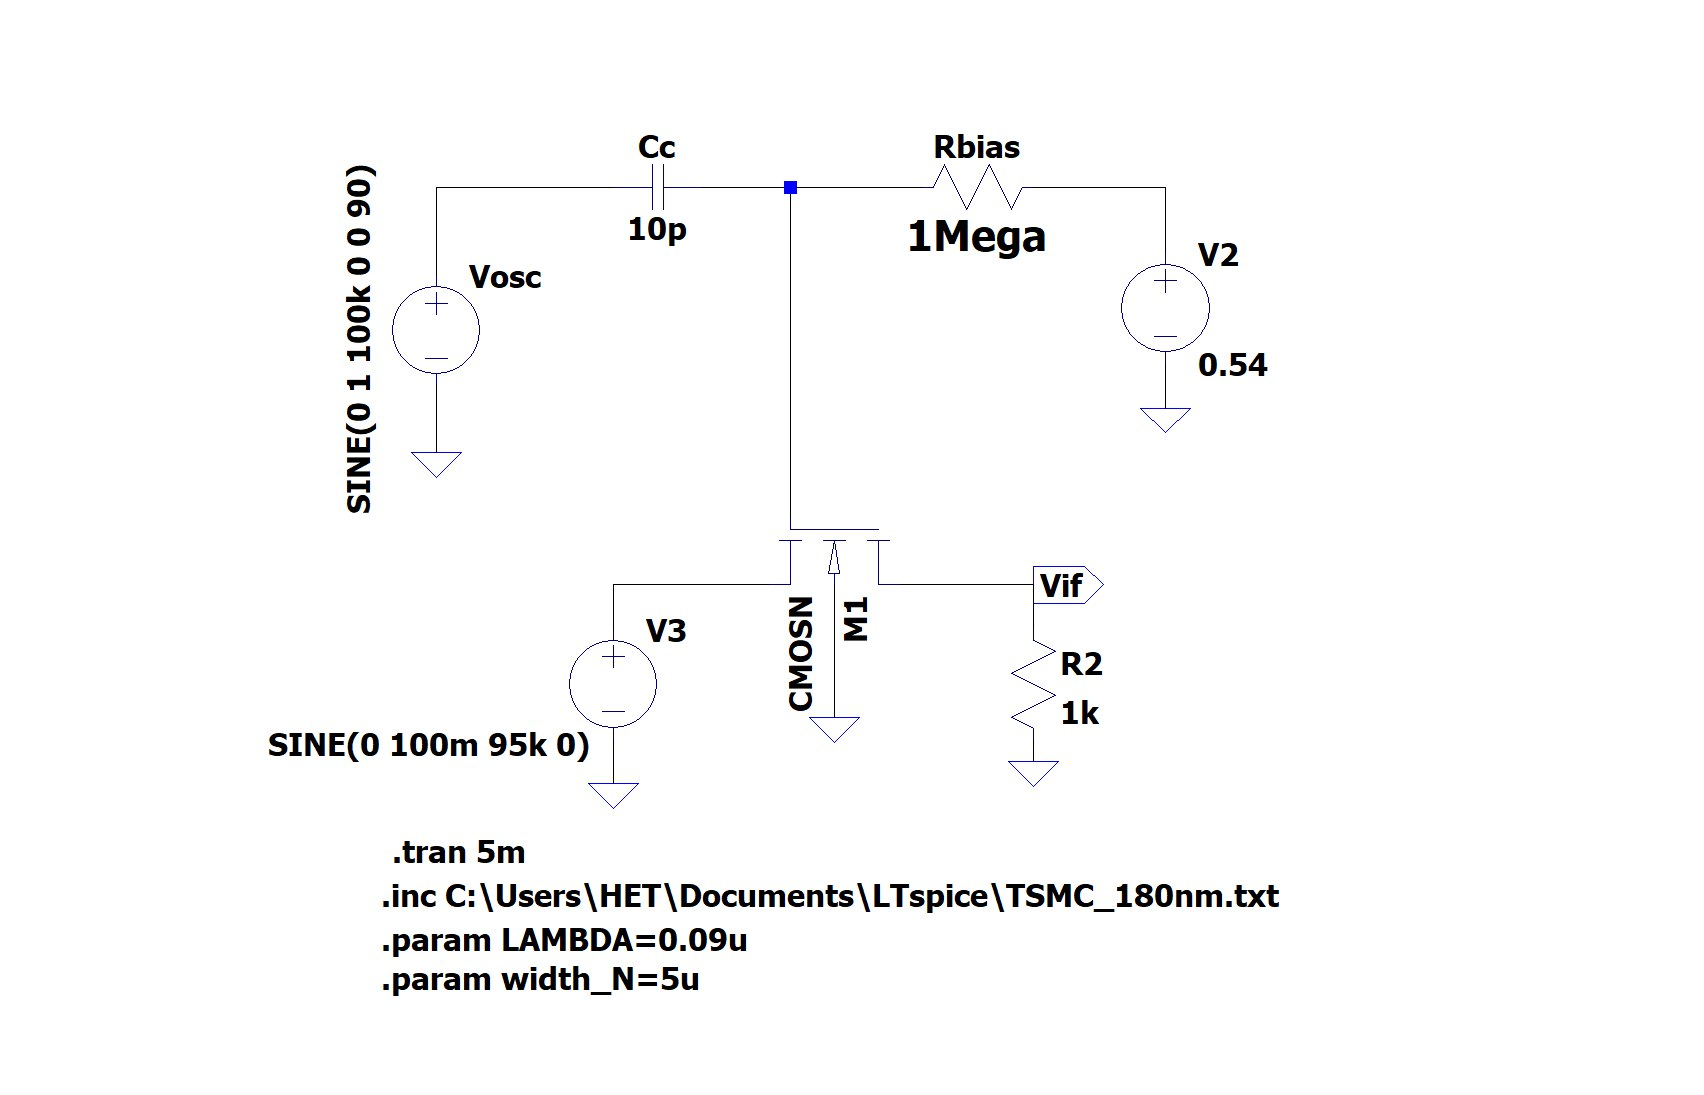
\includegraphics[scale=0.26]{mixer_LT.jpeg}
\caption{LTSpice circuit for Mixer}
\end{figure}

In this design, $R_{BIAS} = 1M\ohm$  and $C_c = 10pF$. Bias voltage is taken to be just greater than the threshold voltage of the MOSFET so that we can
observe a properly on and off switching MOSFET.The NMOS used in our
design has the following characteristics:

\begin{figure}[H]
\centering
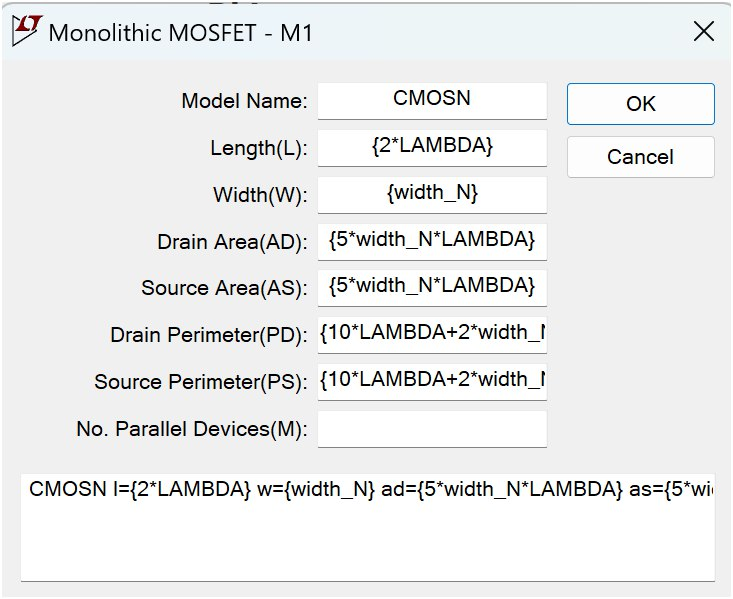
\includegraphics[scale=0.28]{mixer_para.jpeg}
\caption{NMOS Parameters for simulation}
\end{figure}

The following are the time domain plots and FFTs of the
mixer outputs for various input frequencies:

\begin{figure}[H]
\centering
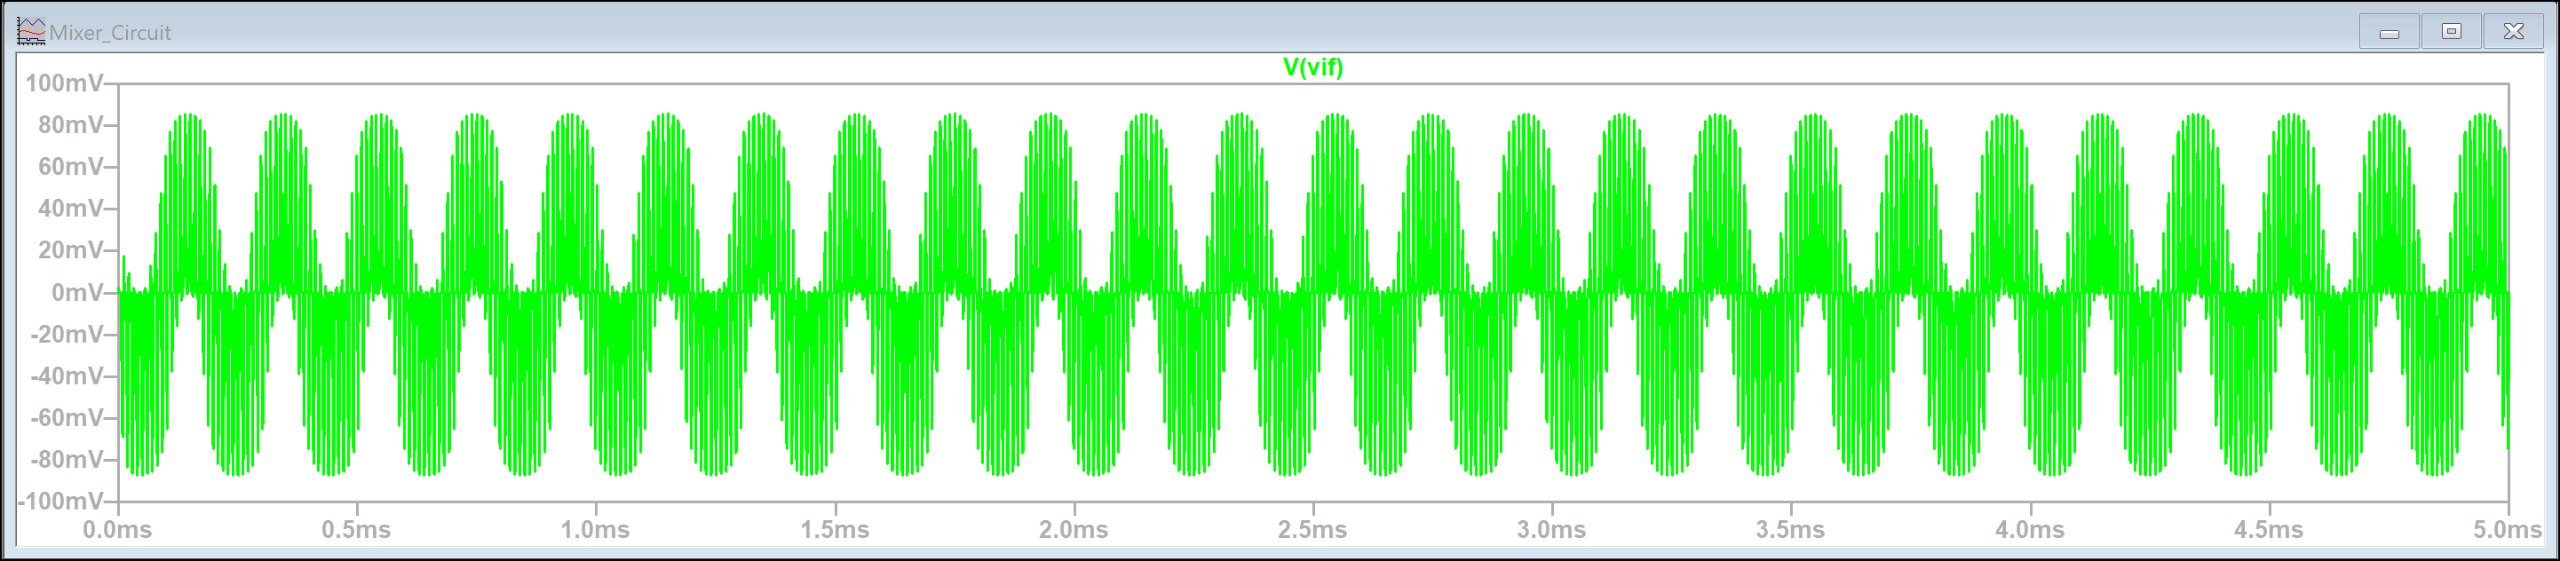
\includegraphics[scale=0.1]{mixer_95.jpeg}
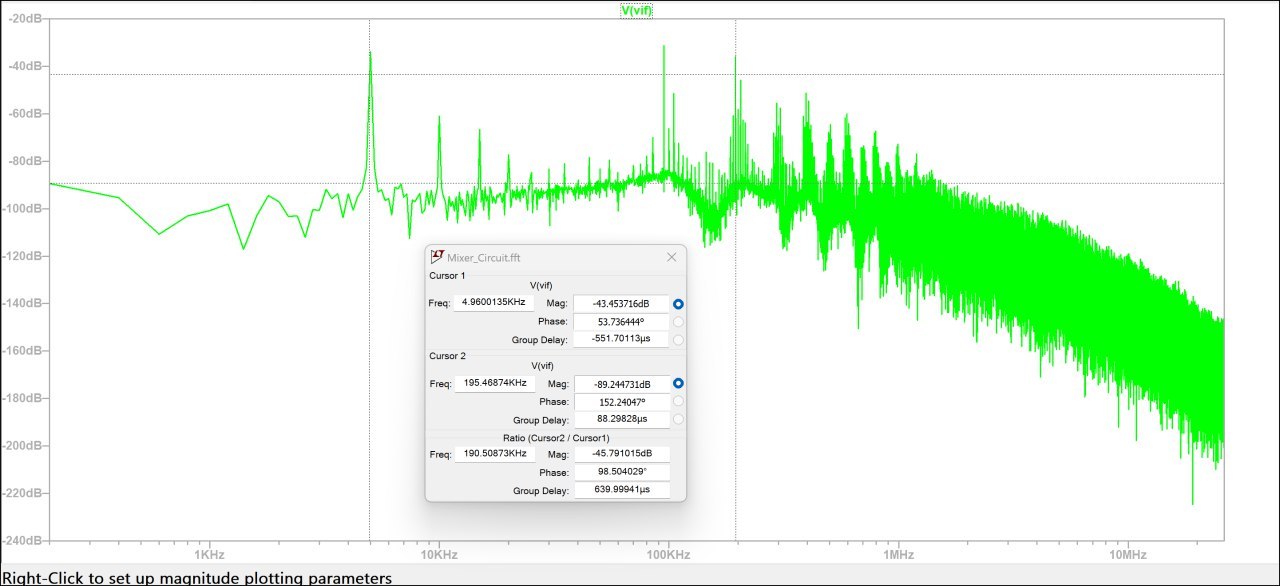
\includegraphics[scale=0.18]{mixer_95fft.png}
\caption{Frequency and Transient response at FIN = 95KHz, we get peaks at 5KHz, 95KHz,
and 195KHz.}
\end{figure}

\begin{figure}[H]
\centering
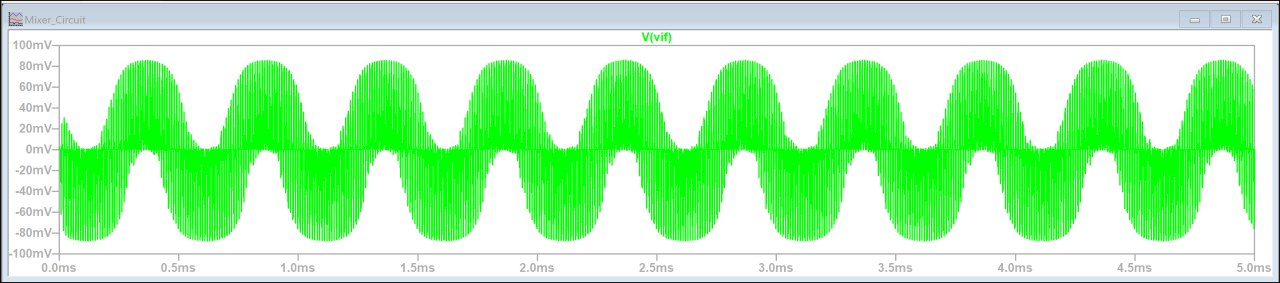
\includegraphics[scale=0.2]{mixer_98.png}
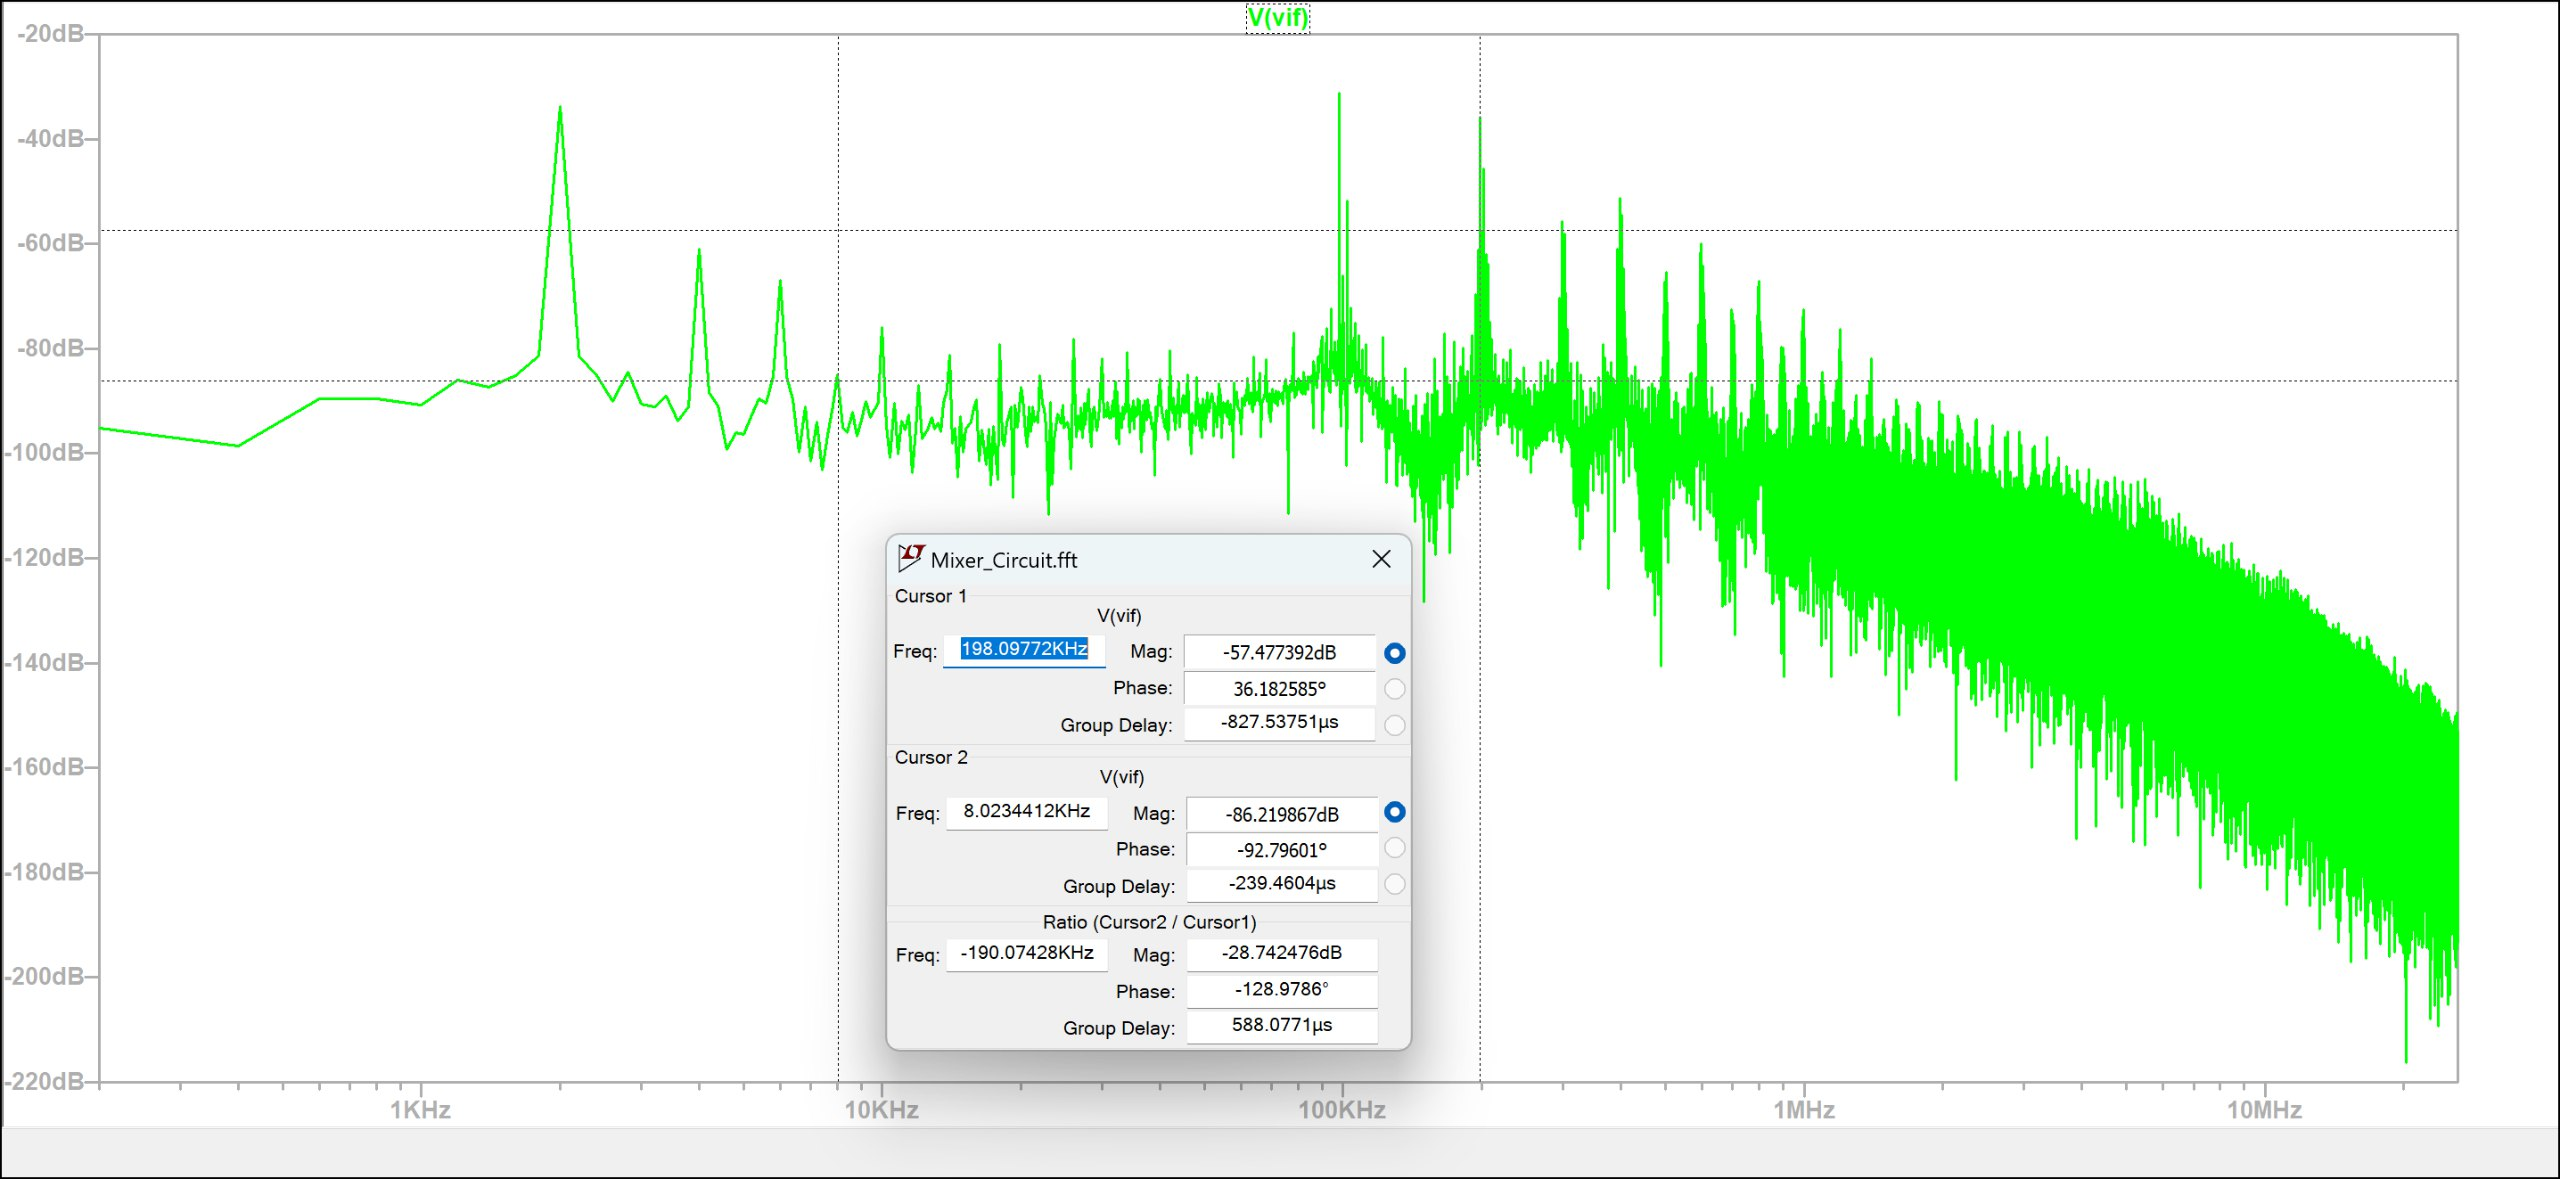
\includegraphics[scale=0.1]{mixer_98fft.jpeg}
\caption{Frequency and Transient response at FIN = 98KHz, we get peaks at 5K 98KHz,
198KHz.}
\end{figure}

\begin{figure}[H]
\centering
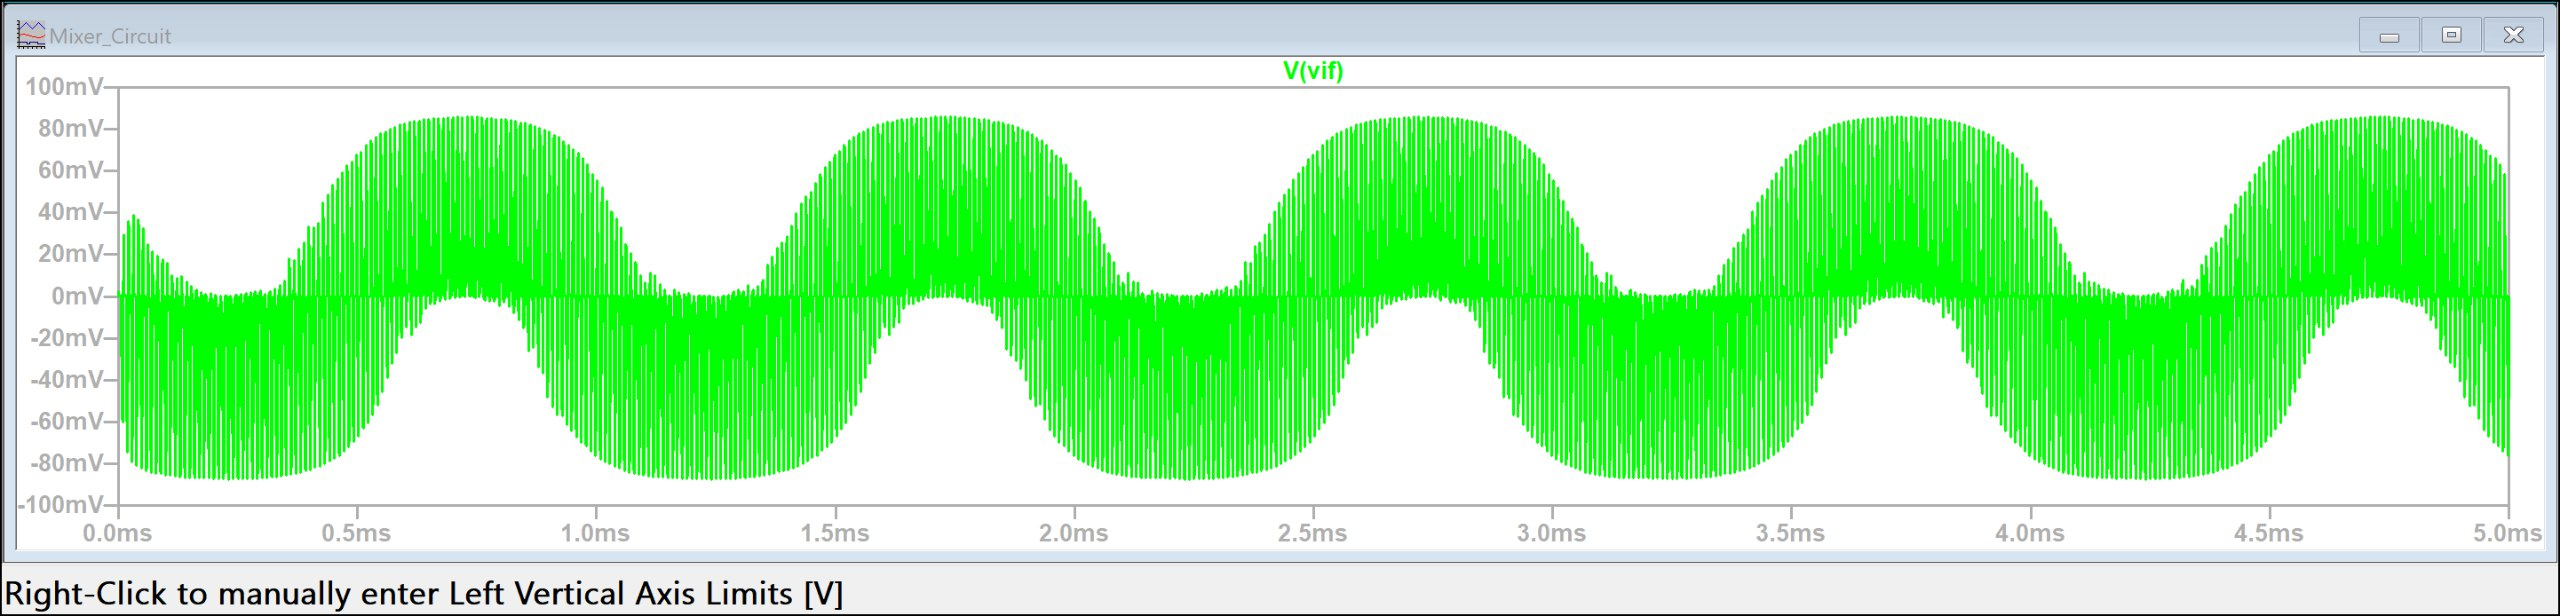
\includegraphics[scale=0.1]{mixer_99.jpeg}
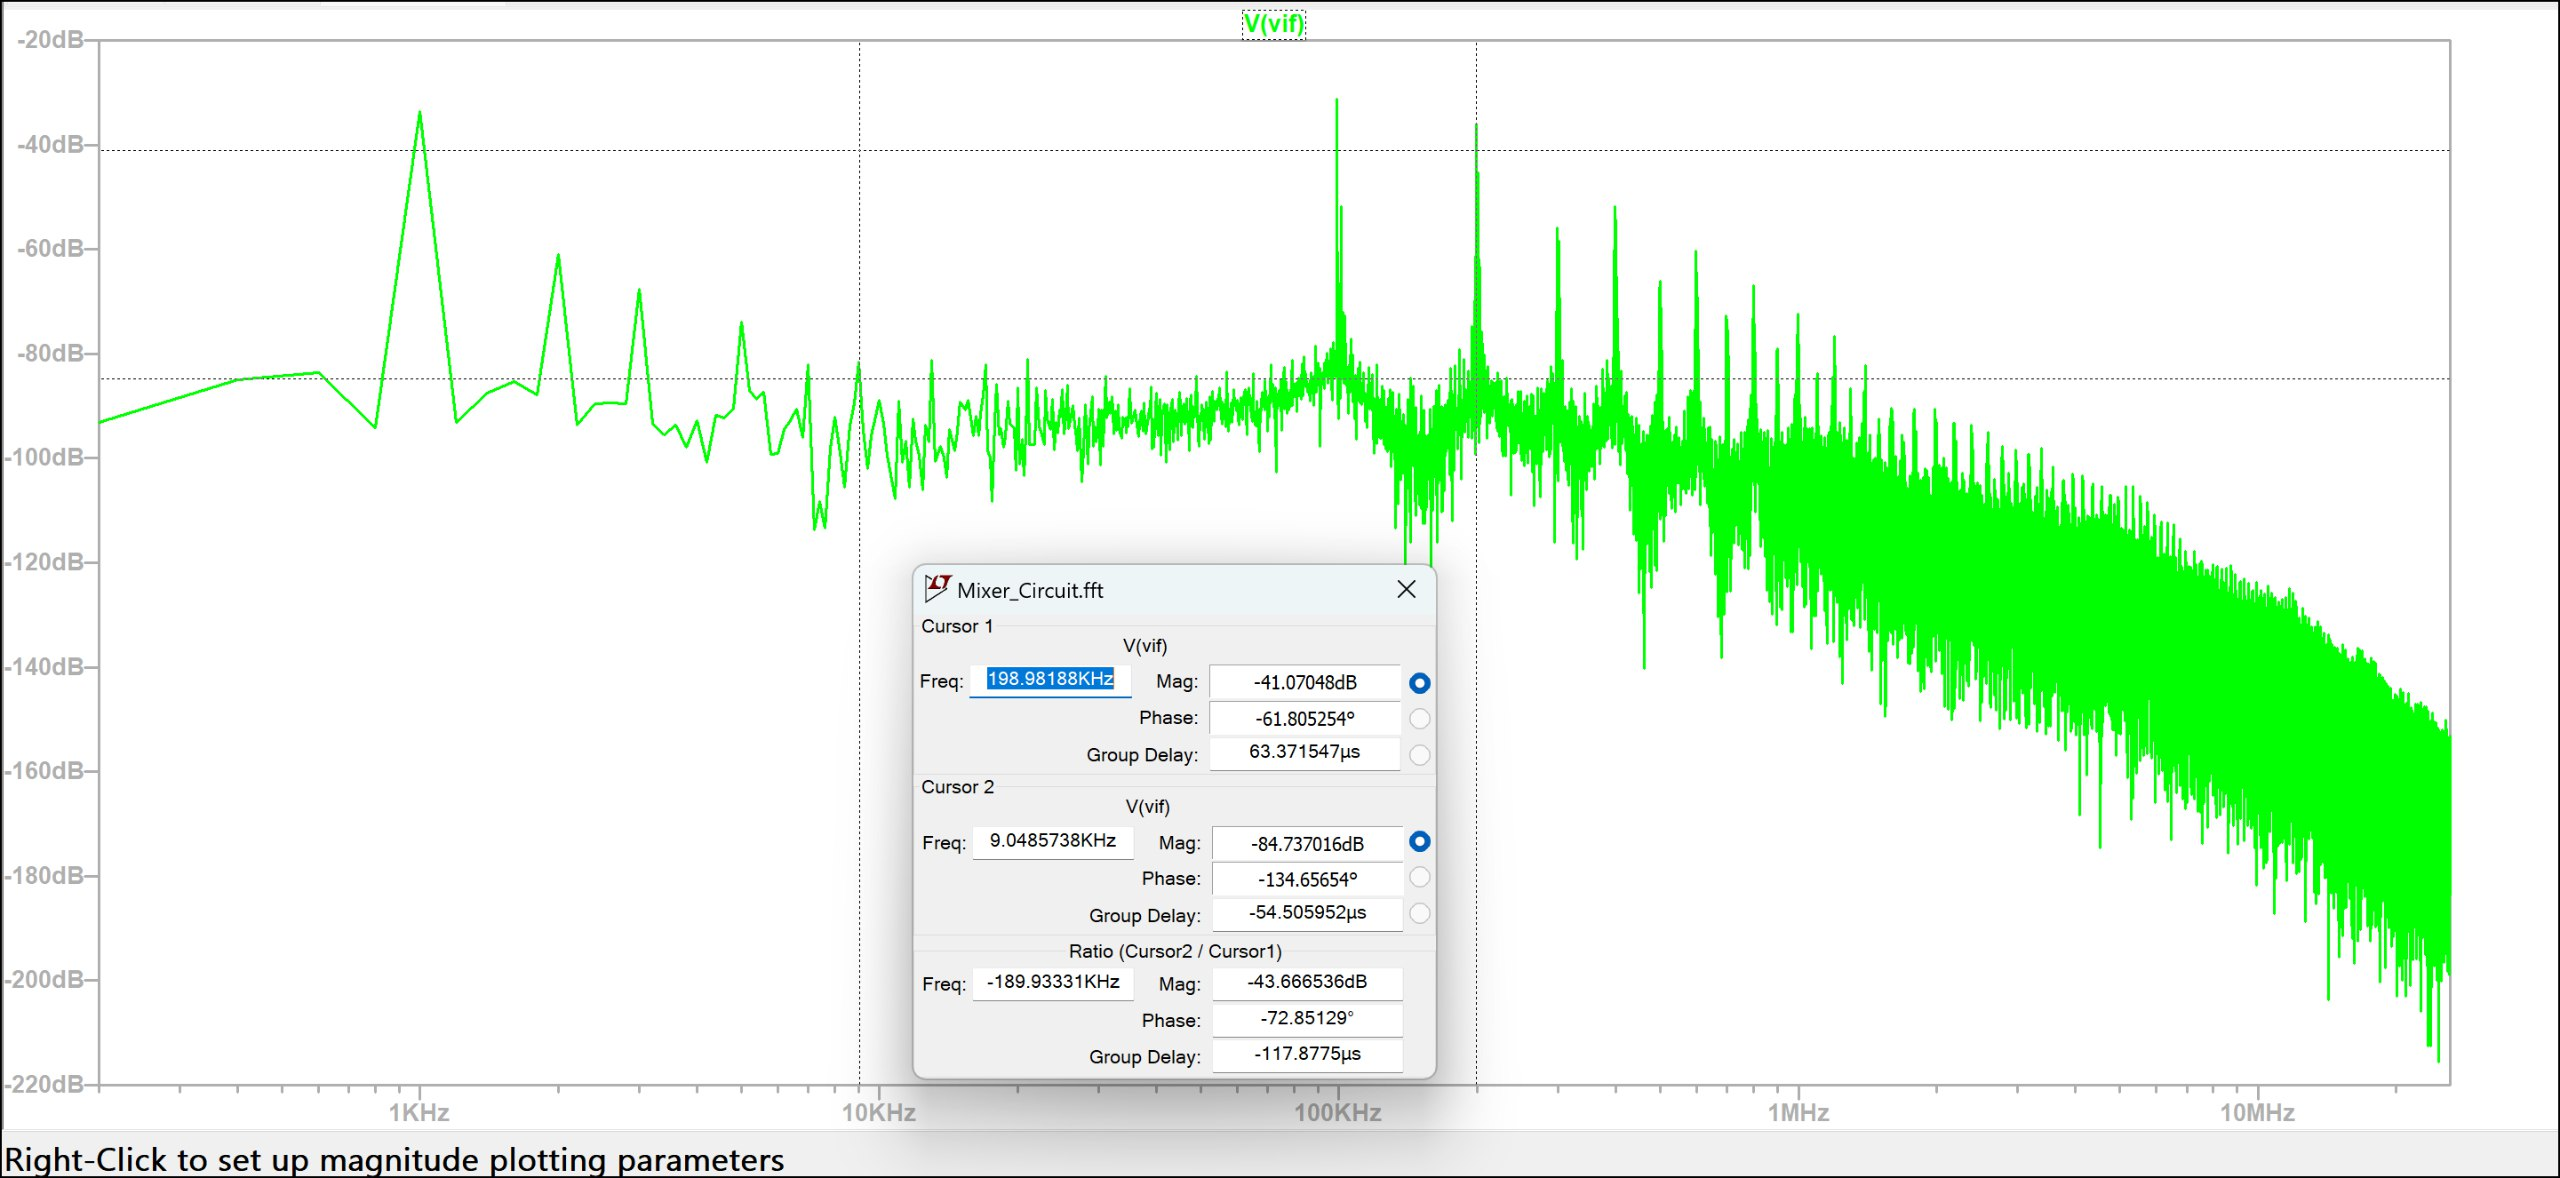
\includegraphics[scale=0.1]{mixer_99fft.jpeg}
\caption{Frequency and Transient response at FIN = 99KHz, we get peaks at 99KHz, 199KHz.}
\end{figure}

\begin{figure}[H]
\centering
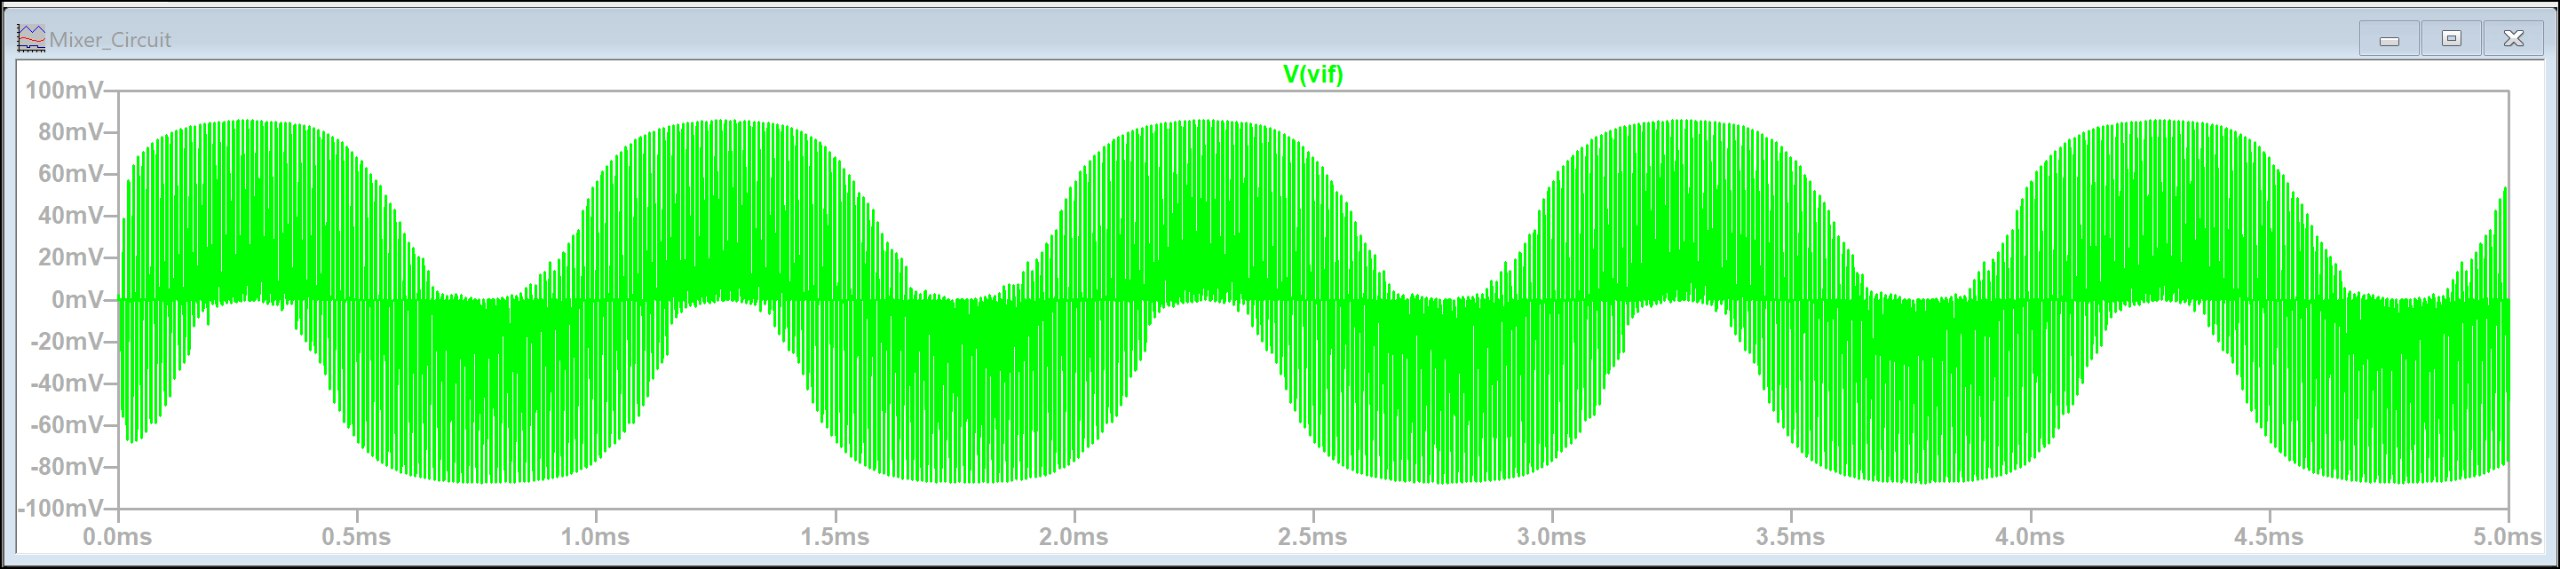
\includegraphics[scale=0.1]{mixer_101.jpeg}
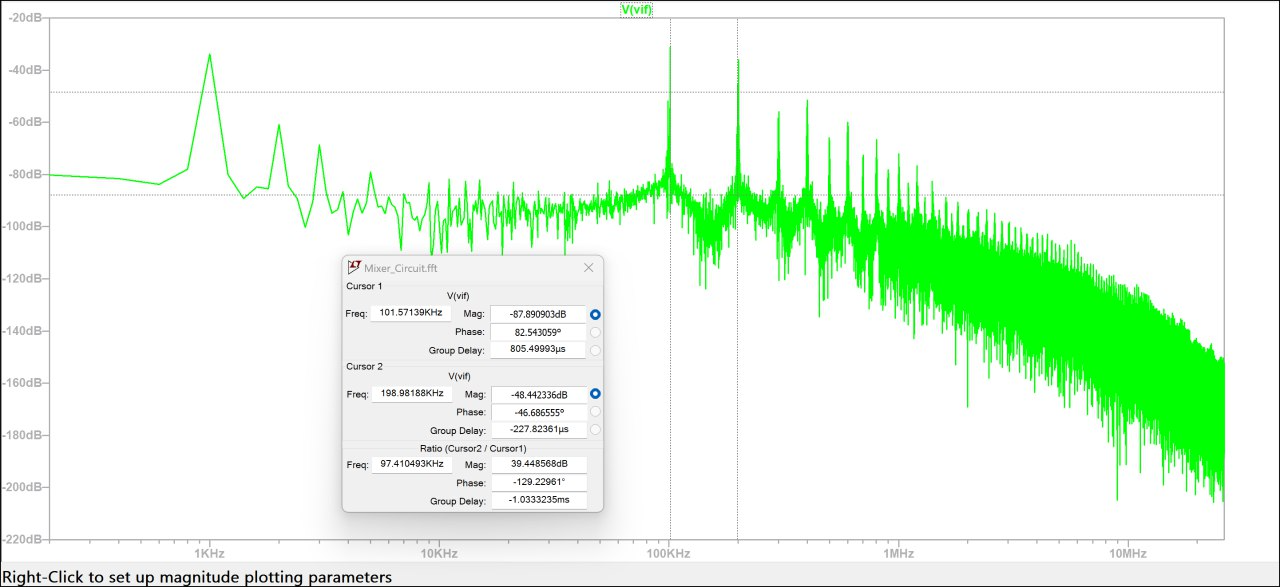
\includegraphics[scale=0.2]{mixer_101fft.png}
\caption{Frequency and Transient response at FIN = 101KHz, we get peaks at 101KHz,201KHz.}
\end{figure}

\begin{figure}[H]
\centering
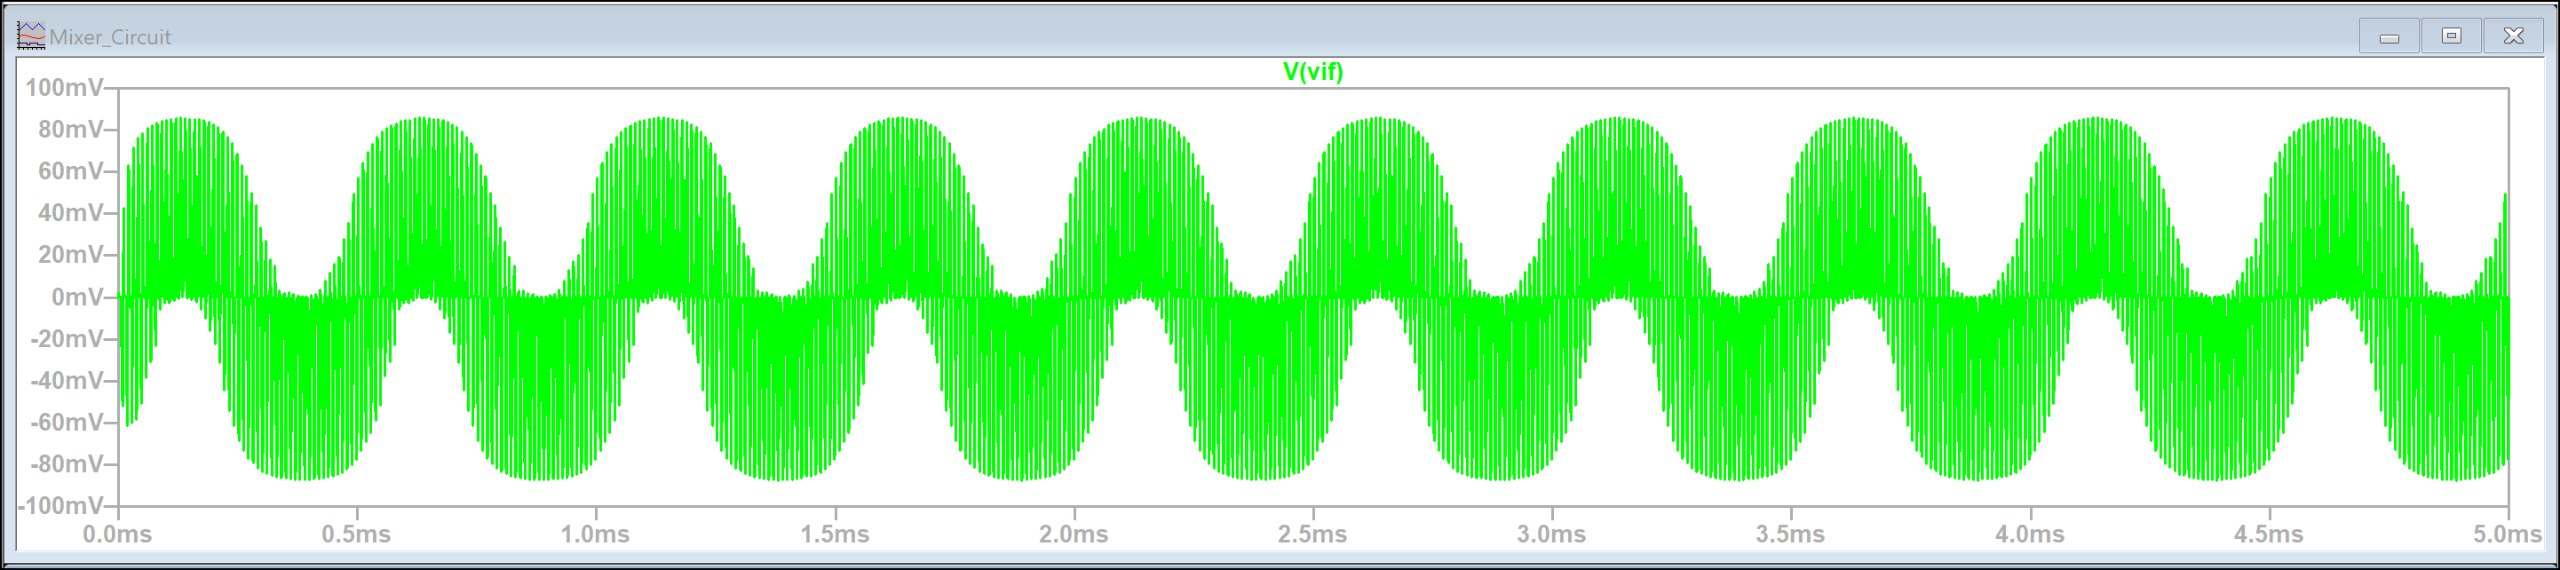
\includegraphics[scale=0.1]{mixer_102.jpeg}
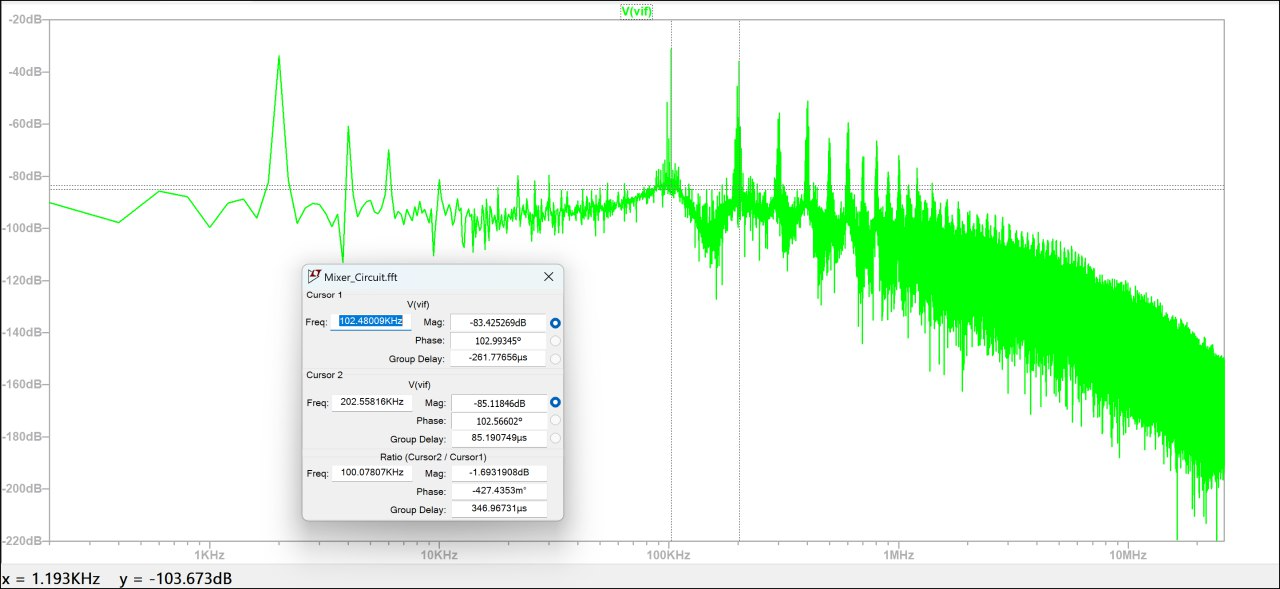
\includegraphics[scale=0.18]{mixer_102fft.png}
\caption{Frequency and Transient response  at FIN = 102KHz, we get peaks at 102KHz,
202KHz.}
\end{figure}

\begin{figure}[H]
\centering
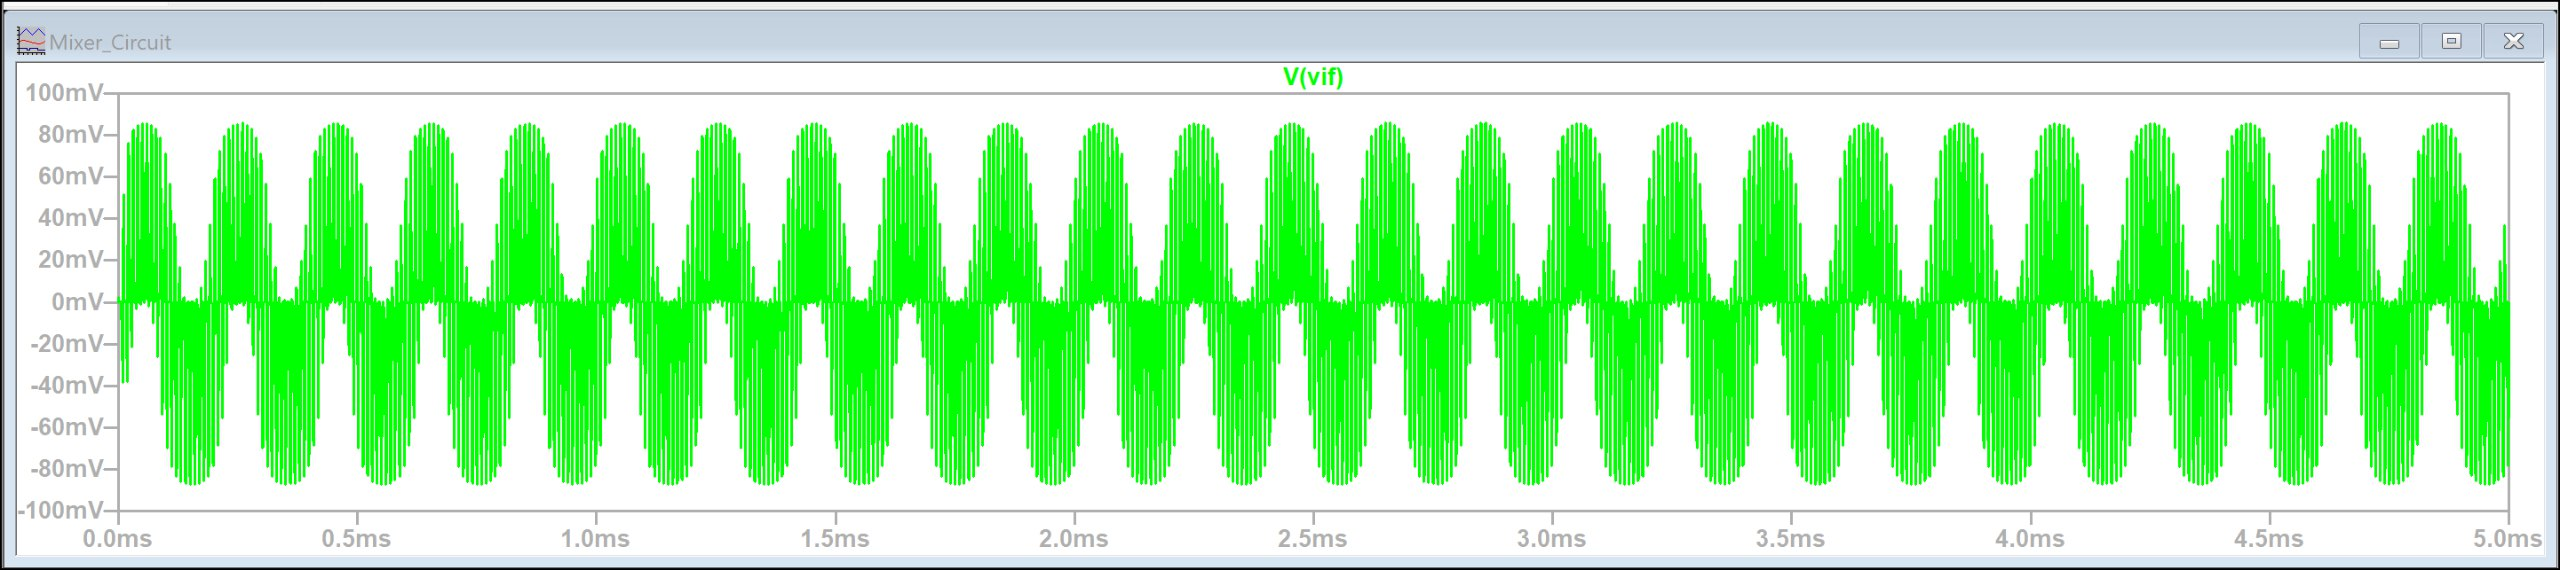
\includegraphics[scale=0.08]{mixer_105.jpeg}
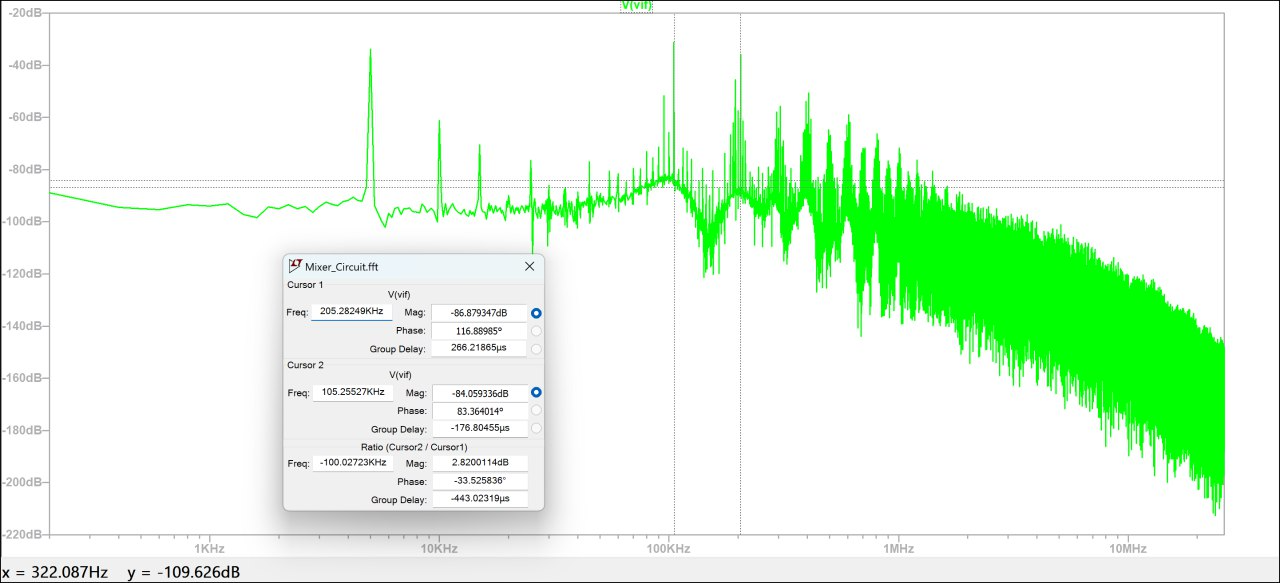
\includegraphics[scale=0.15]{mixer_105fft.png}
\caption{Frequency and Transient response at FIN = 105KHz, we get peaks at 105 KHz,
205KHz.}
\end{figure}

\section{Low Pass Filter}

A low-pass filter is an electronic circuit that allows low-frequency signals to pass through while attenuating (reducing) high-frequency components. Its operation is based on the frequency-dependent impedance of its components—typically resistors and capacitors in an RC configuration.

\subsection{Working of Low Pass Filter}

\begin{itemize}
    \item At low frequencies, the capacitor behaves like an open circuit, allowing signals to pass through with minimal attenuation.
    \item At high frequencies, the capacitor acts as a short circuit, diverting the signal away from the output.
    \item The RC low-pass filter functions as a frequency-dependent voltage divider: 
    \begin{itemize}
        \item At low frequencies, most of the input voltage appears across the output (across the capacitor).
        \item At high frequencies, more voltage is dropped across the resistor, resulting in reduced output amplitude.
    \end{itemize}
    \item The resistor controls the current flow into the capacitor and influences the capacitor's charging and discharging rate.
\end{itemize}

\subsection{Determination of Cutoff Frequency,R and C}

The cutoff frequency \( f_c \) is the point where the filter starts to attenuate higher-frequency signals significantly. It is determined using the resistor \( R \) and capacitor \( C \) values, given by the formula:

\begin{equation}
f_c = \frac{1}{2\pi RC}
\end{equation}

\subsubsection{Formulae}
$$Intensity = 20\log_{10}|H(\omega)|$$
where $H(\omega)$ is the transfer function in frequency response of system
$$V_{out} = \frac{X_c}{X_c+R}V_{in} = \frac{\frac{1}{j\omega C}}{\frac{1}{j\omega C}+R}V_{in}$$
where Capacitor Impedence,$X_c = \frac{1}{j\omega C}$
$$\frac{V_{out}}{V_{in}}=\frac{1}{1+j\omega RC}$$
Amplitude Gain$$= -20\log_{10}\frac{1}{1+j\omega RC}$$

\subsubsection{Calculations}
$$f_c = \frac{1}{2\pi RC}= 2KHz$$
We have taken $R = 2K\ohm$
$$\Rightarrow C = \frac{1}{2\pi Rf_c} = \frac{1}{2\pi \times2\times10^3\times2\times10^3} = 3.979\times10^{-8}F\approx39.79nF$$

\subsection{Simulations}

\begin{figure}[H]
\centering
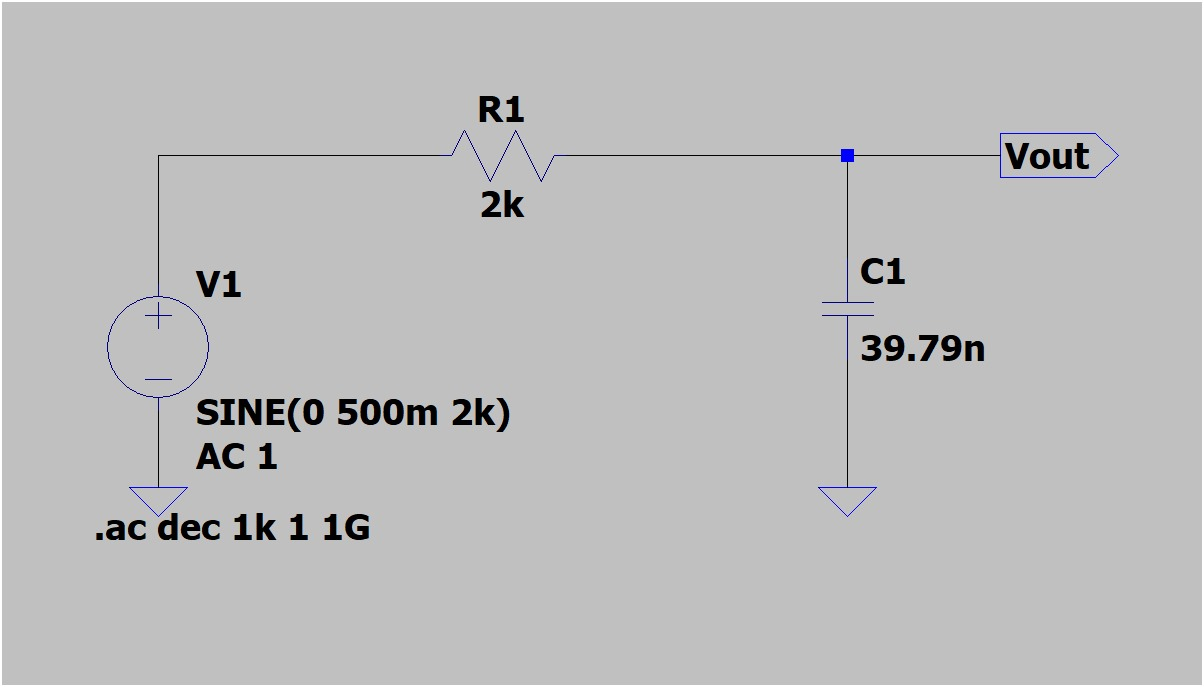
\includegraphics[scale=0.25]{lowpass_LT_circuit.jpg}
\caption{ Realizing RC low pass filter with cut off frequency 2KHz on
LTSPICE.}
\end{figure}
\subsubsection{Frequency Response}

The frequency response shows a change in behavior near 1.99 KHz(cutoff frequency), marking significant attenuation as it approaches 1 kHz (input signal frequency).

\begin{figure}[H]
\centering
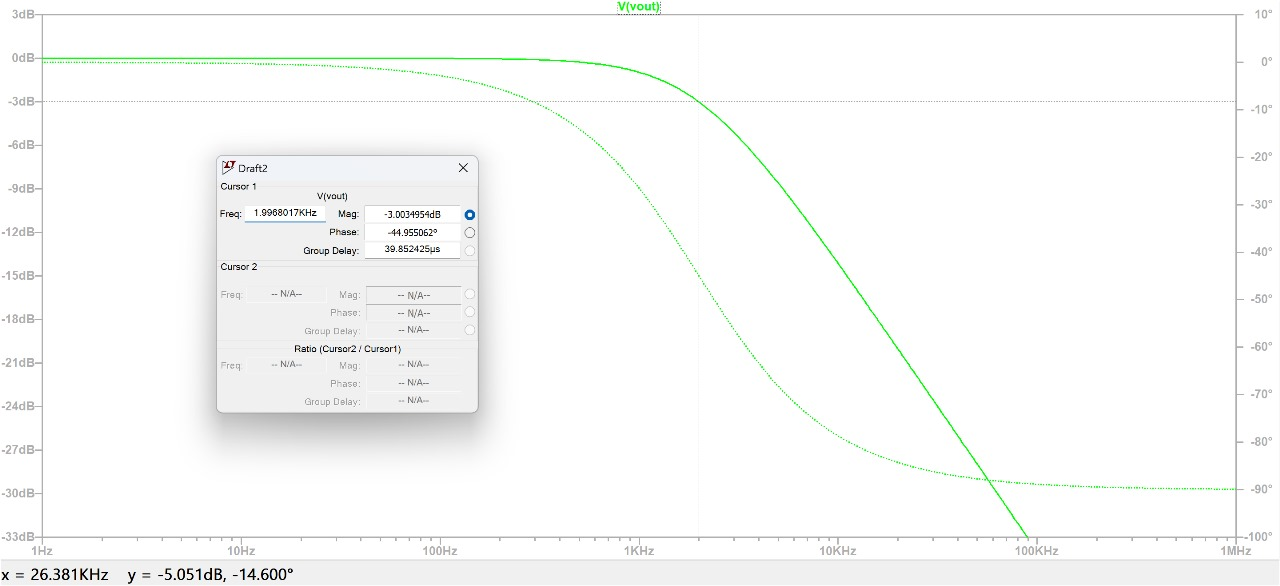
\includegraphics[scale=0.25]{lowpass_spice1.jpg}
\caption{Frequency response of RC low pass filter}
\end{figure}

\begin{figure}[H]
\centering
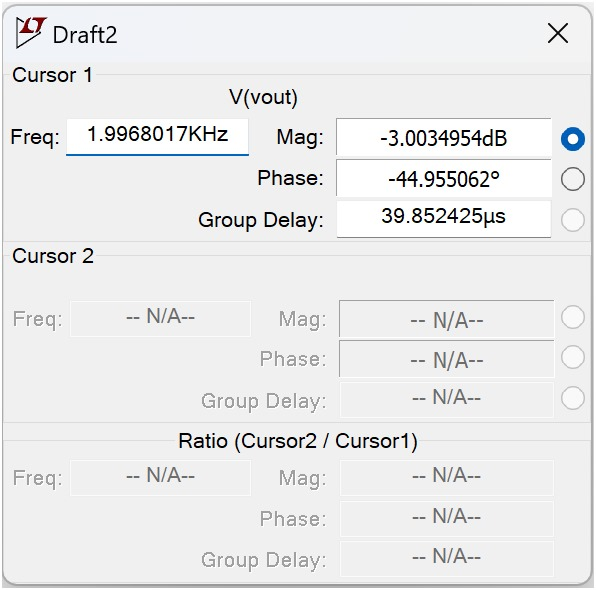
\includegraphics[scale=0.25]{lowpass_3db.jpg}
\caption{we get -3dB frequency at 1.99KHz.}
\end{figure}

\subsubsection{Transient Response}
The transient response illustrates how the filter behaves under different frequency inputs (e.g., 20 kHz, 10 kHz, 1 kHz), showing varying degrees of attenuation and signal shaping.

\begin{figure}[H]
\centering
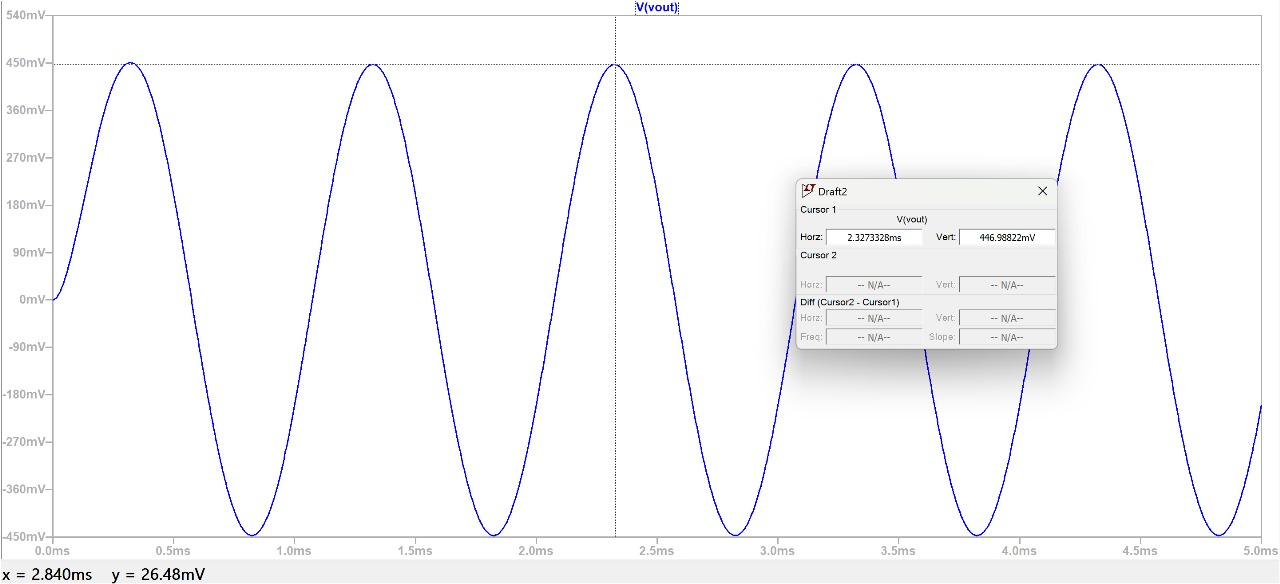
\includegraphics[scale=0.25]{lowpass_spice2.jpg}
\caption{Frequency = 1k}
\end{figure}

\begin{figure}[H]
\centering
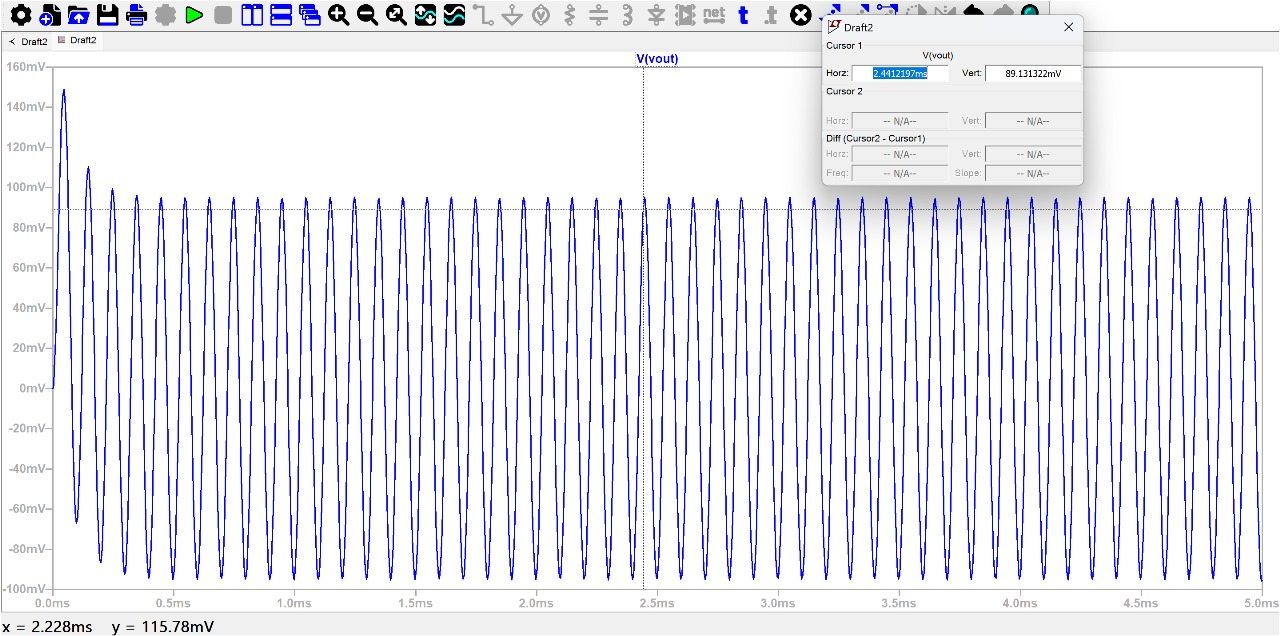
\includegraphics[scale=0.25]{lowpass_spice3.jpg}
\caption{Frequency = 10k}
\end{figure}

\begin{figure}[H]
\centering
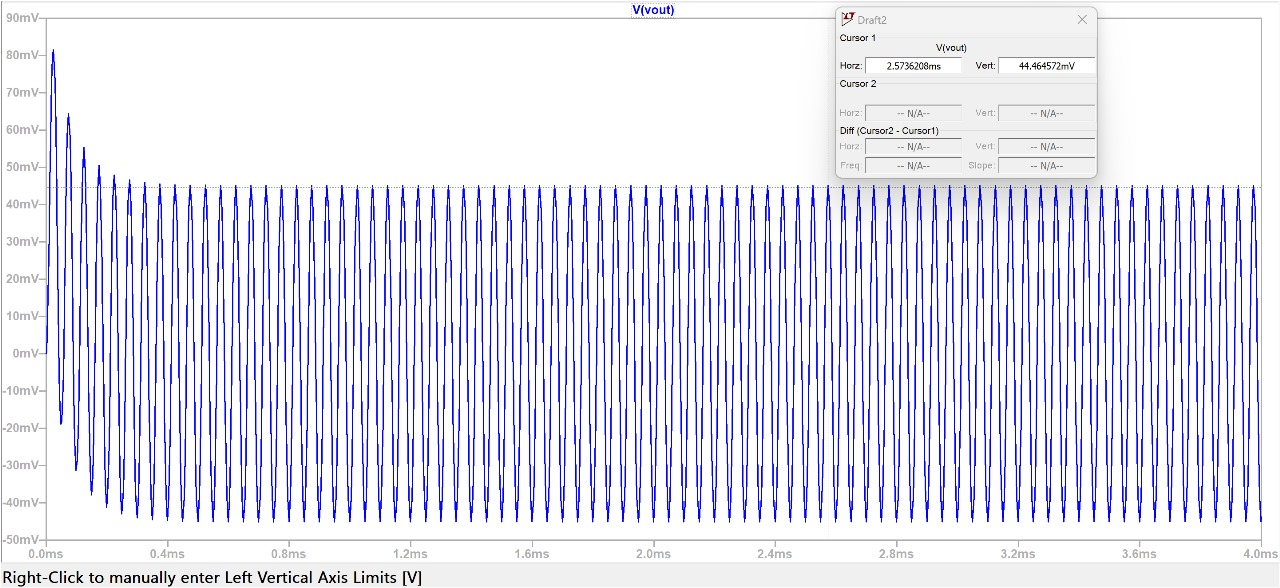
\includegraphics[scale=0.25]{lowpass_spice4.jpg}
\caption{Frequency = 20k}
\end{figure}

\section{Complete circuit prototype design}
The first part of our circuit is oscillator, which takes DC
voltage as input for VDD, VSS of Op-amps. The output of this
oscillator consists of 2 signals, one sine and other cosine, both
at a phase difference of $90\degree$. This signals act as oscillator
signals in mixer, the cosine output wave is input for the Inphase mixer, and sine wave for quadrature-phase mixer. The
input signal for the mixer’s, are given from the wave
generator. The output of the mixer is passed through the low
pass filter to filter out any frequency greater than 2KHz.
Finally, we have 2 output signalsfrom the low pass filters, one
in-phase component and other quadrature phase component.

\subsection{Complete circuit realized on LTSPICE}
\begin{figure*}[!t]
\centering
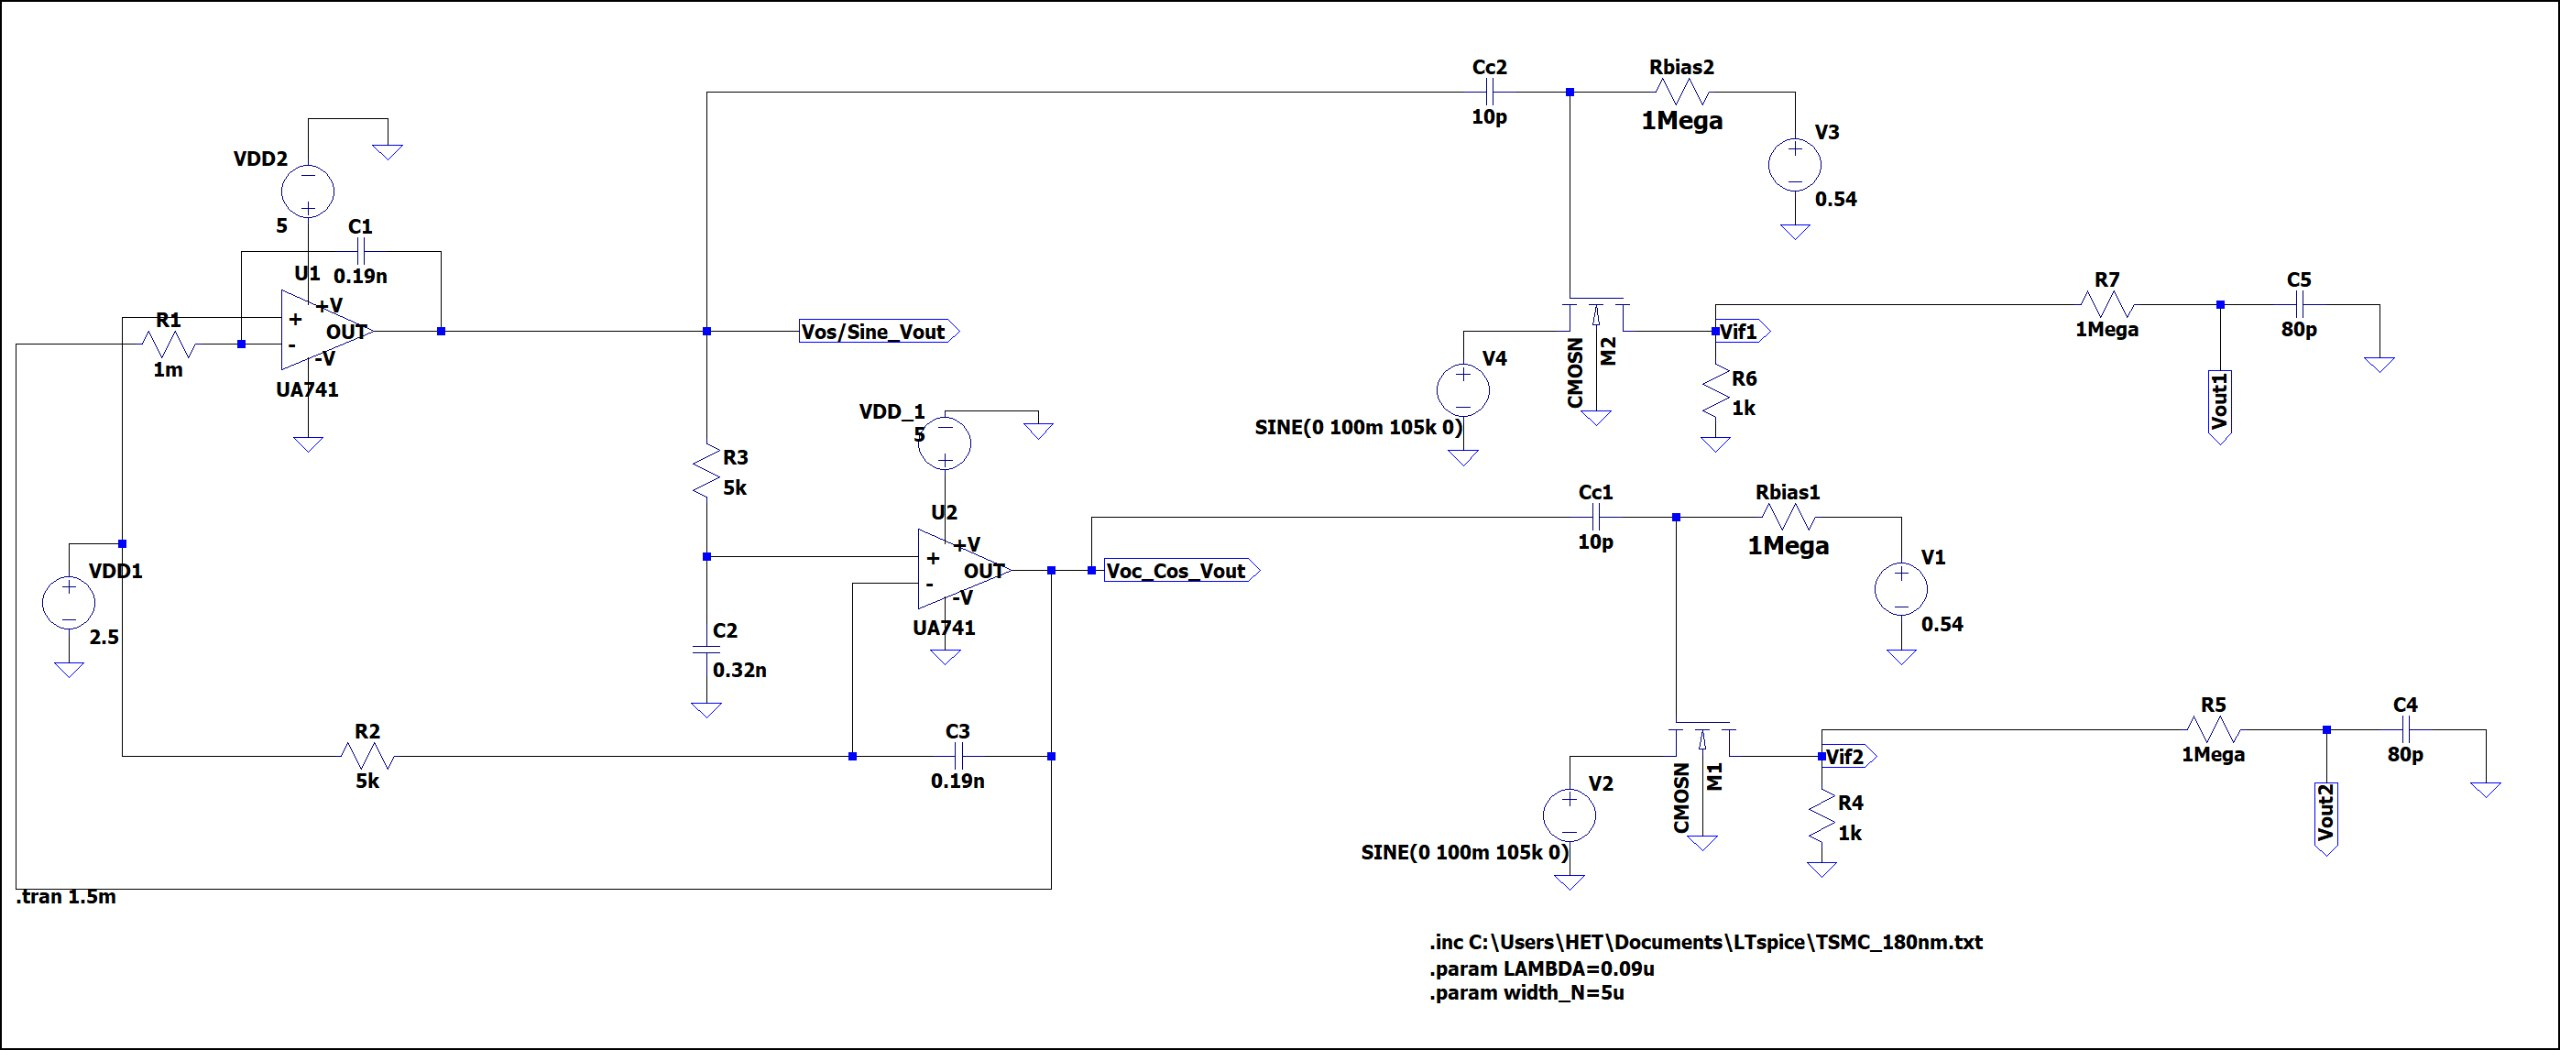
\includegraphics[scale=0.2]{final_lt.jpeg}
\caption{LTSPICE circuit for the complete QDC prototype}
\end{figure*}

\begin{figure}[H]
\centering
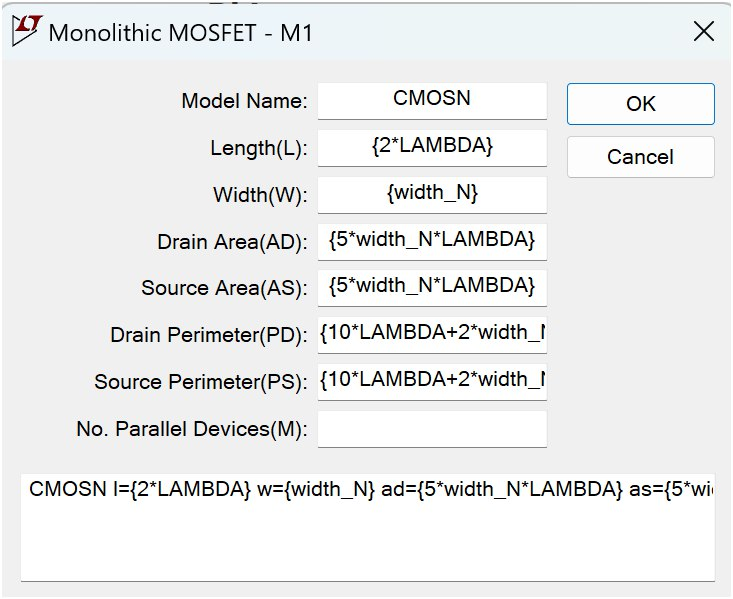
\includegraphics[scale=0.25]{mixer_para.jpeg}
\caption{NMOS Paramerters}
\end{figure}

\subsection{Simulation Plots and Results}

\begin{figure}[H]
\centering
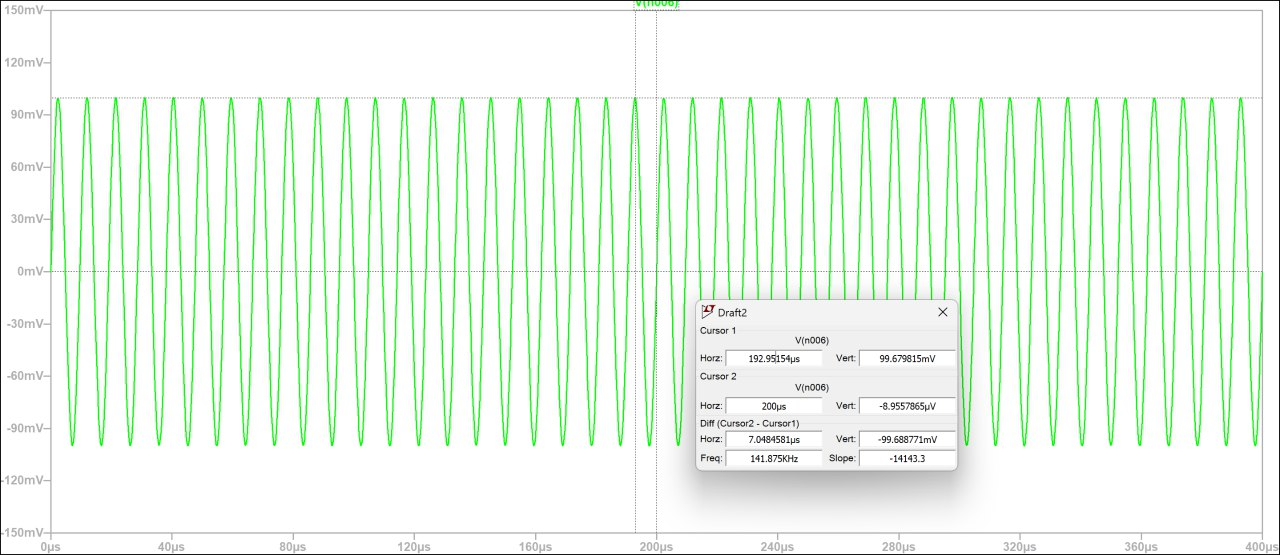
\includegraphics[scale=0.2]{final_in.png}
\caption{Input signal with amplitude 100mV, frequency 105KHz.}
\end{figure}

\begin{figure}[H]
\centering
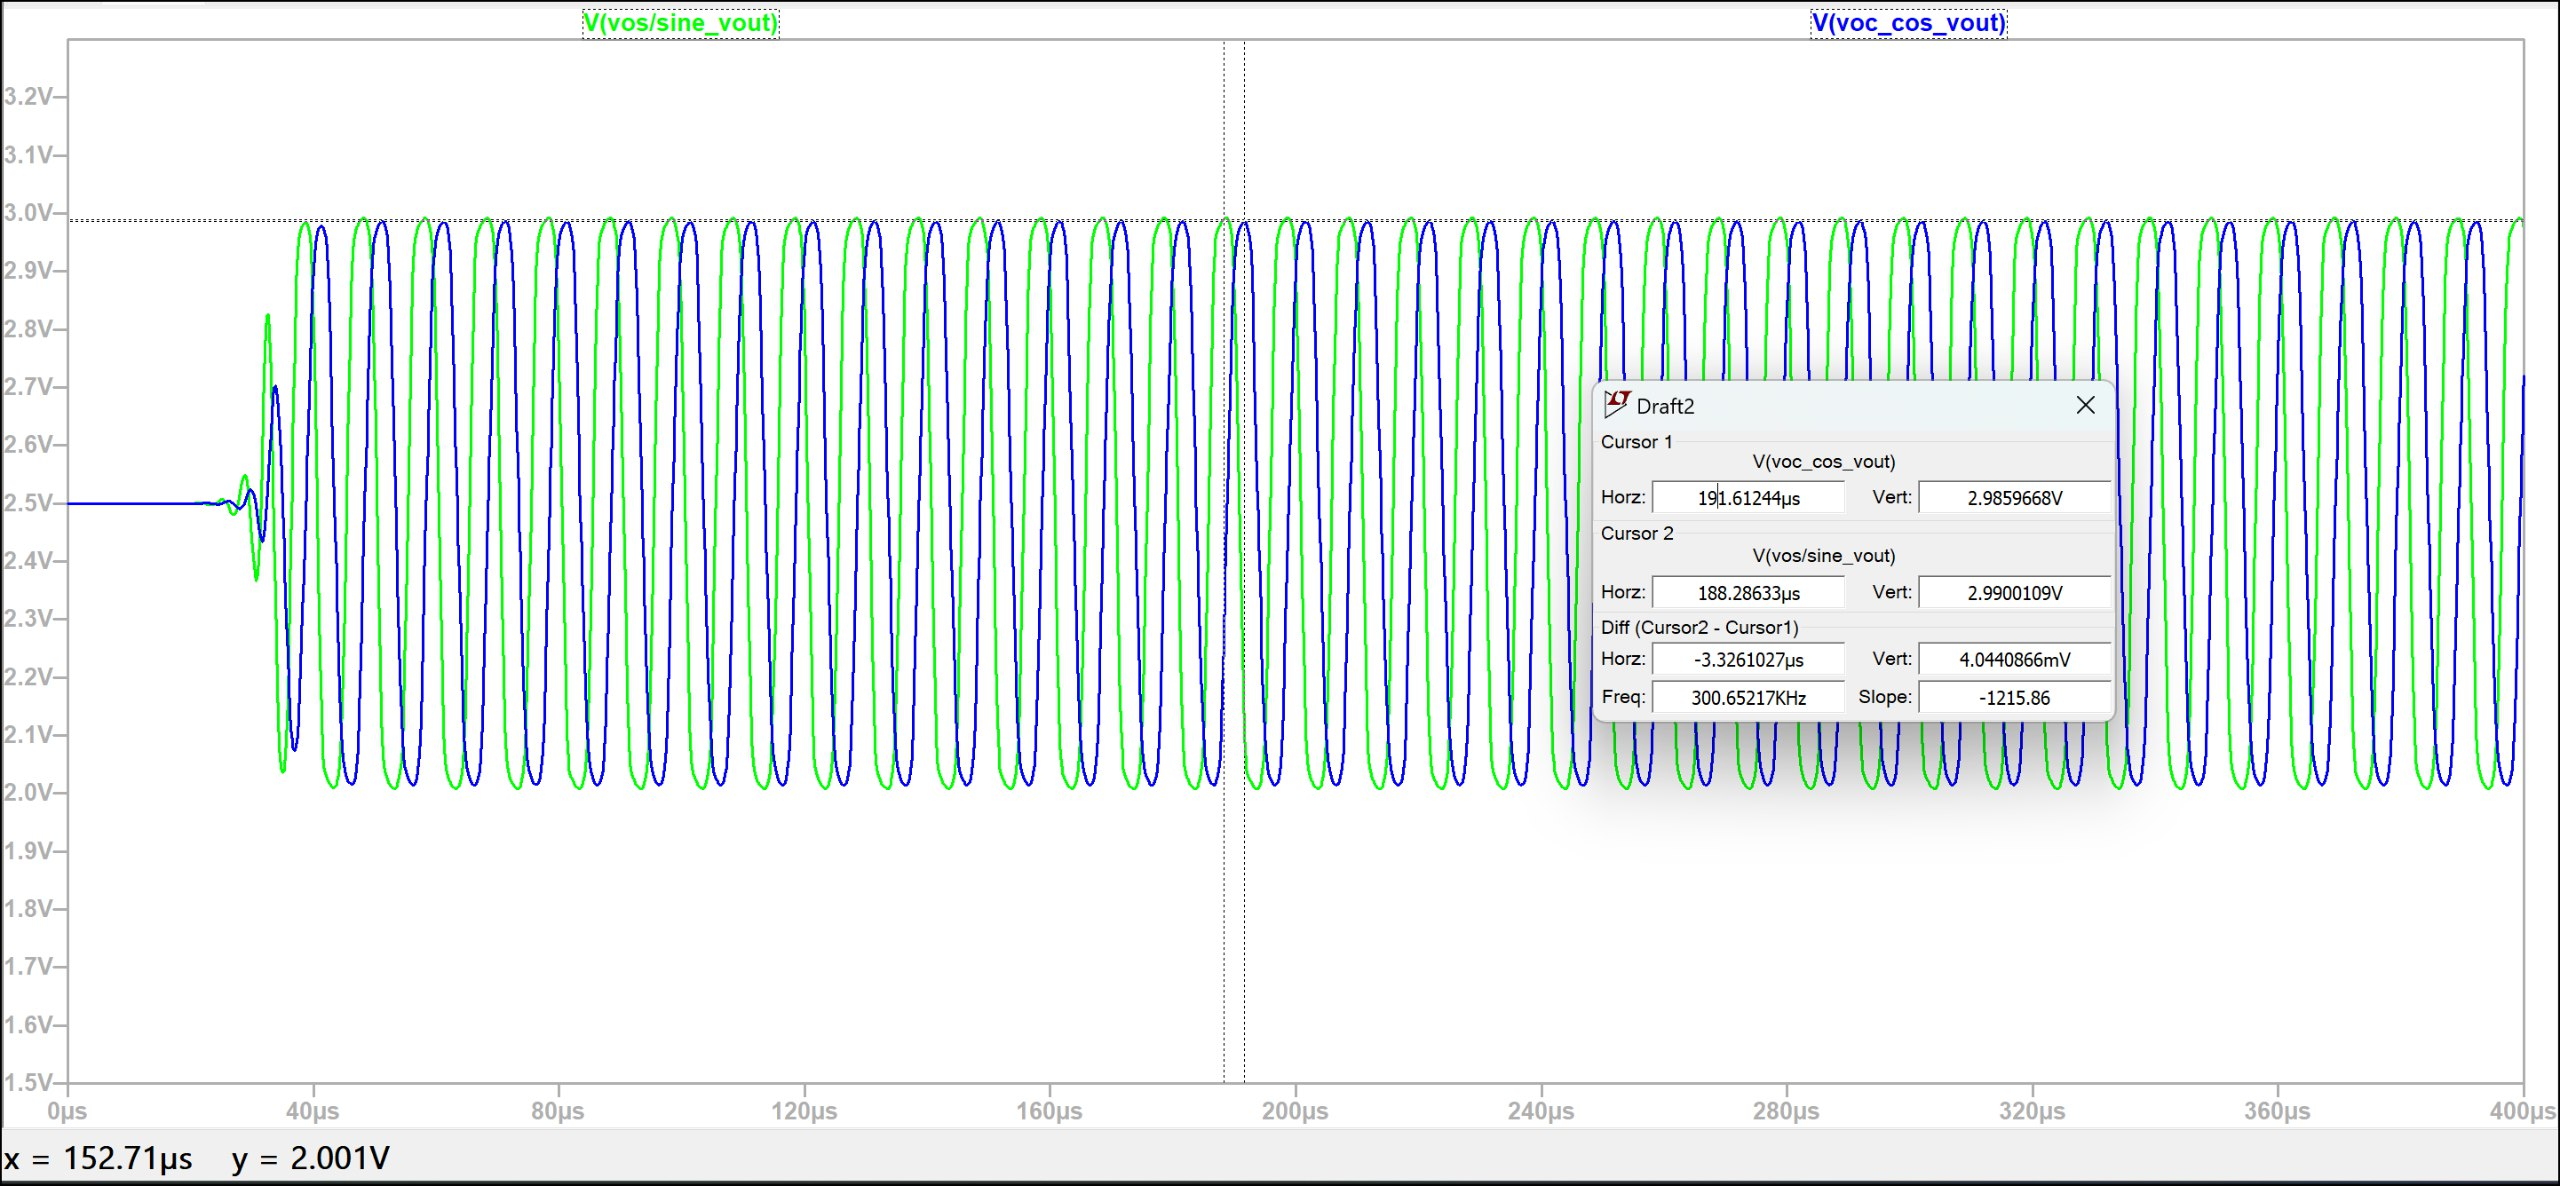
\includegraphics[scale=0.1]{final_osc.jpeg}
\caption{ Transient plots for in-phase and quadrature-phase
components of the oscillator, showing 90° phase shift}
\end{figure}

\begin{figure}[H]
\centering
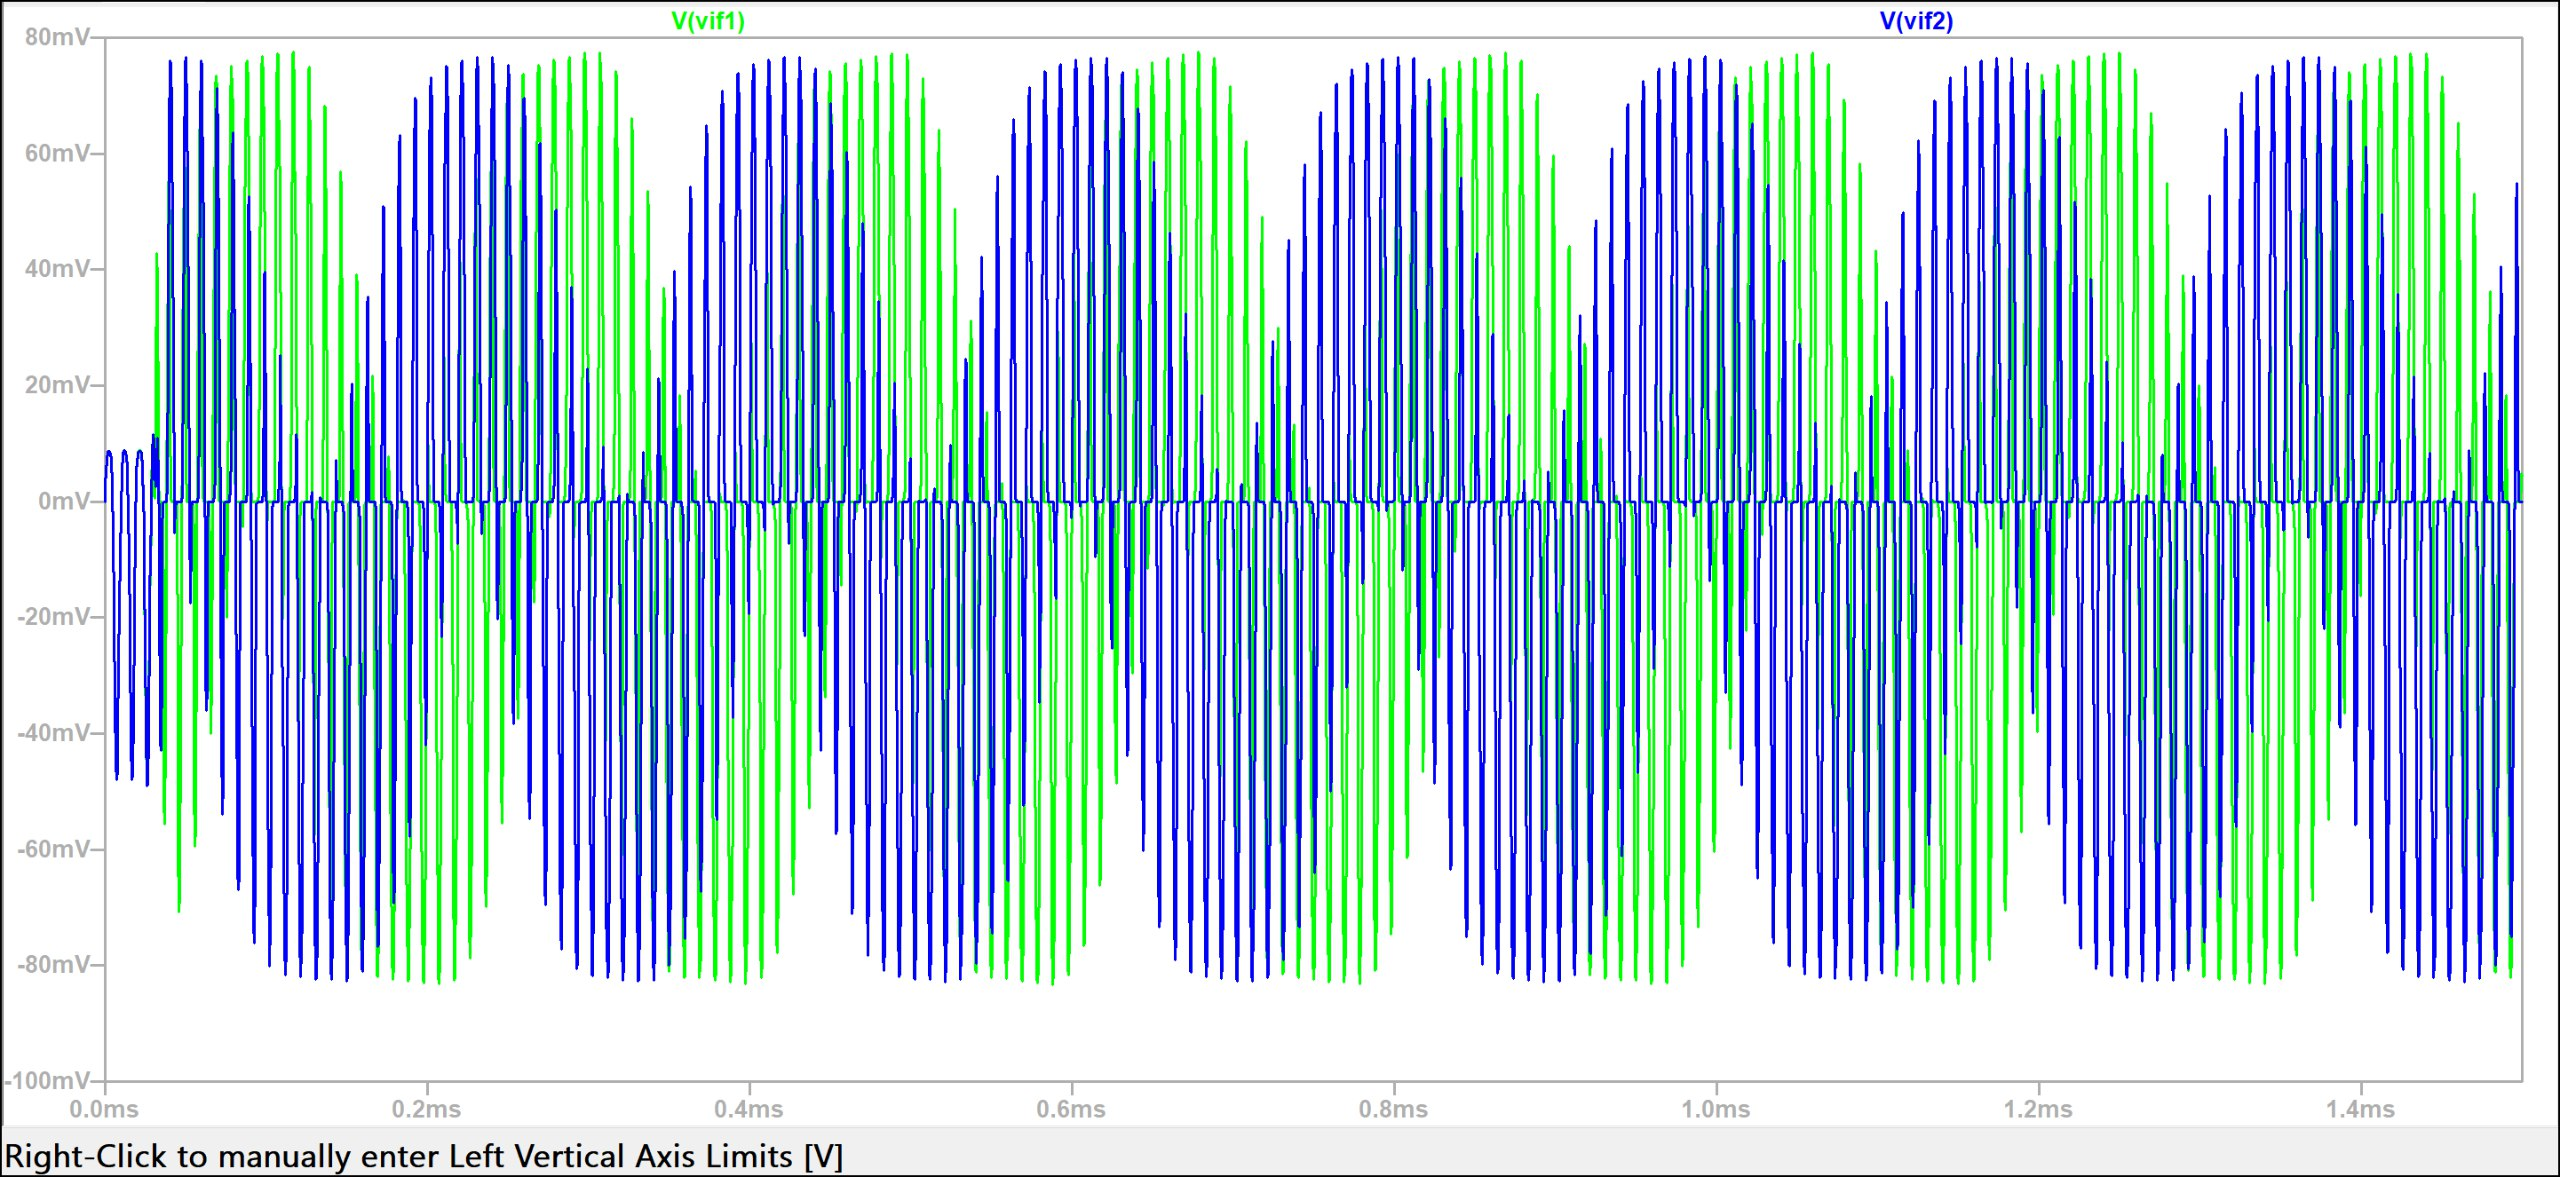
\includegraphics[scale=0.1]{final_mixer.jpeg}
\caption{ Output of mixer when the above-mentioned output signals of
oscillator and $V_{in}$ are given input to the mixer.}
\end{figure}

\begin{figure}[H]
\centering
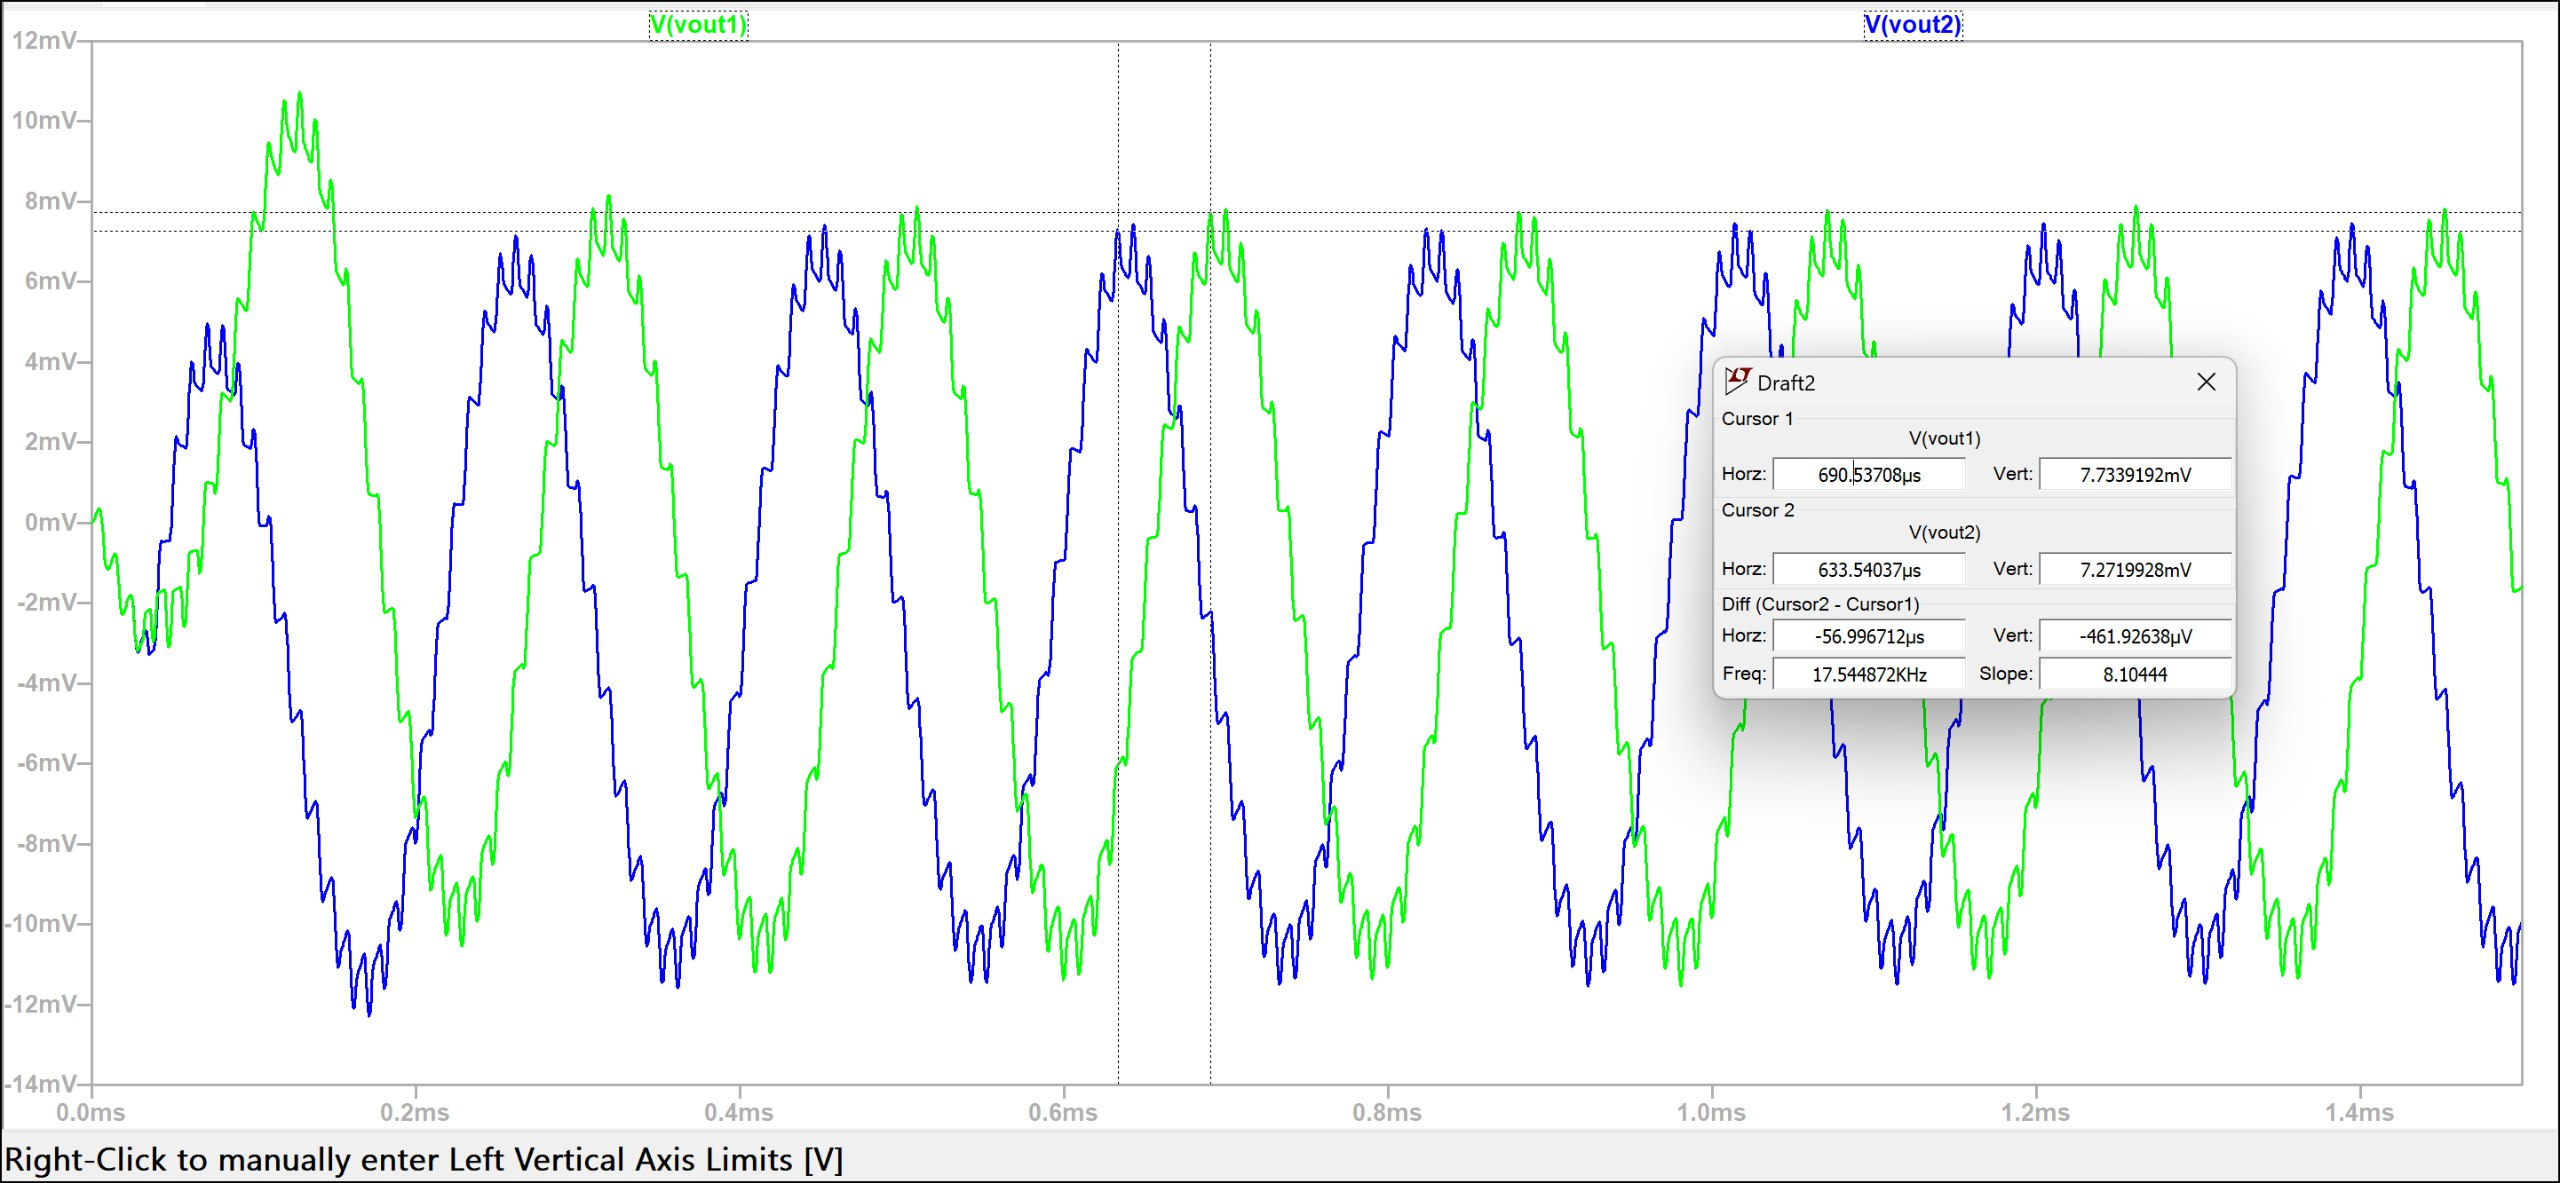
\includegraphics[scale=0.1]{final_out.jpeg}
\caption{Final output plot of QDC showing in-phase and
quadrature-phase components of input signal with phase difference
of 90°}
\end{figure}

\begin{figure}[H]
\centering
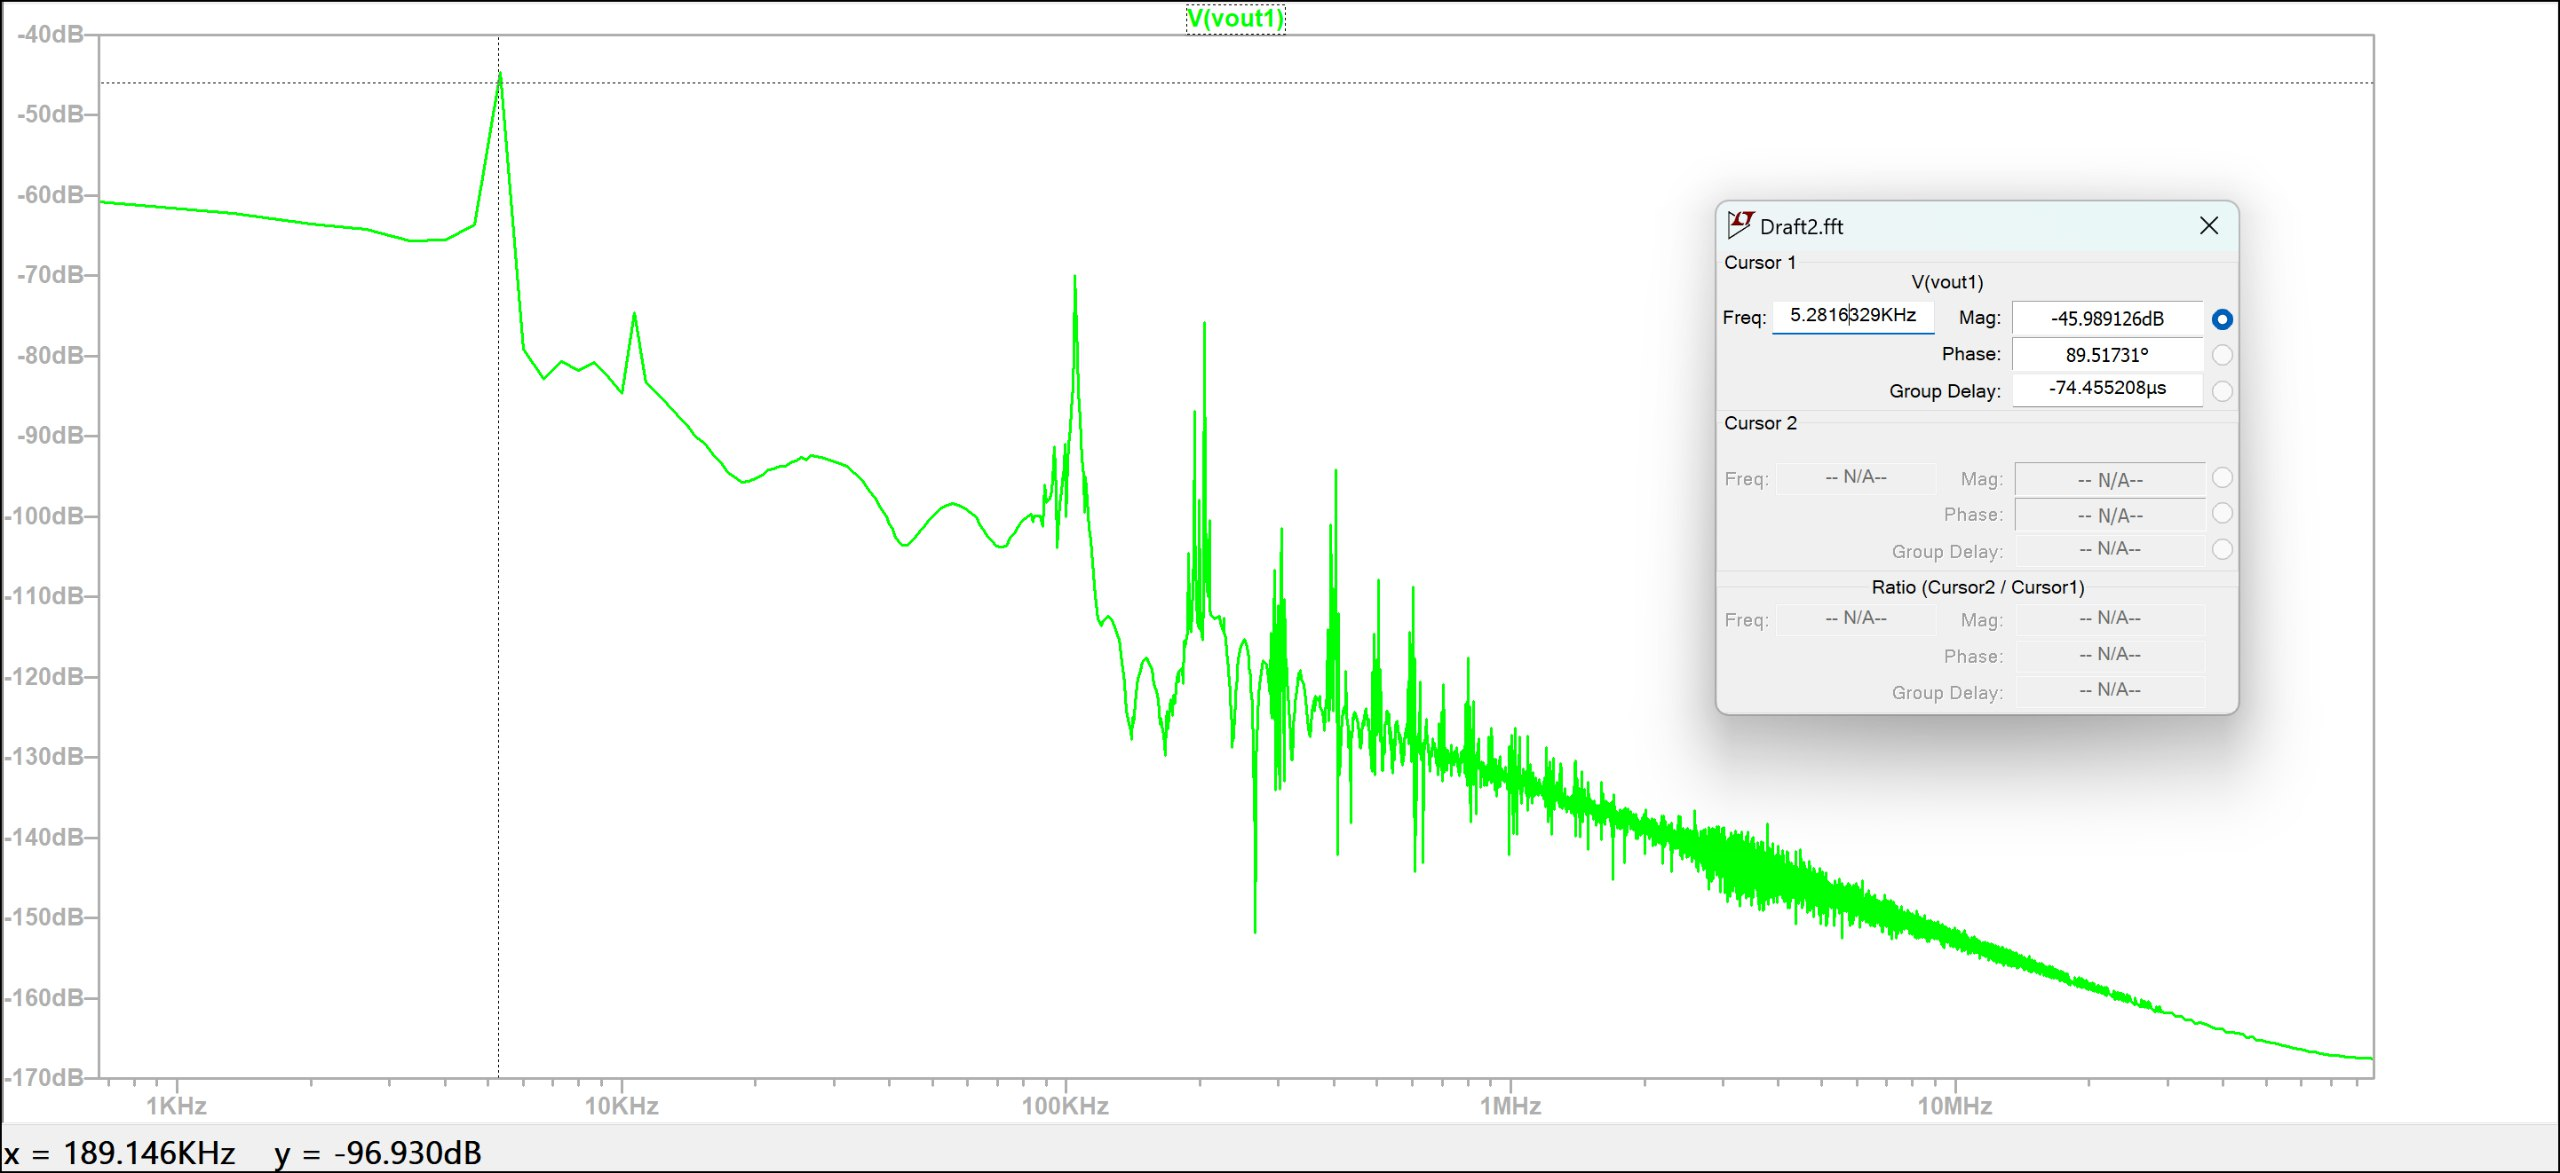
\includegraphics[scale=0.1]{final_fft1.jpeg}
\caption{ FFT plot of quadrature-phase output}
\end{figure}

\begin{figure}[H]
\centering
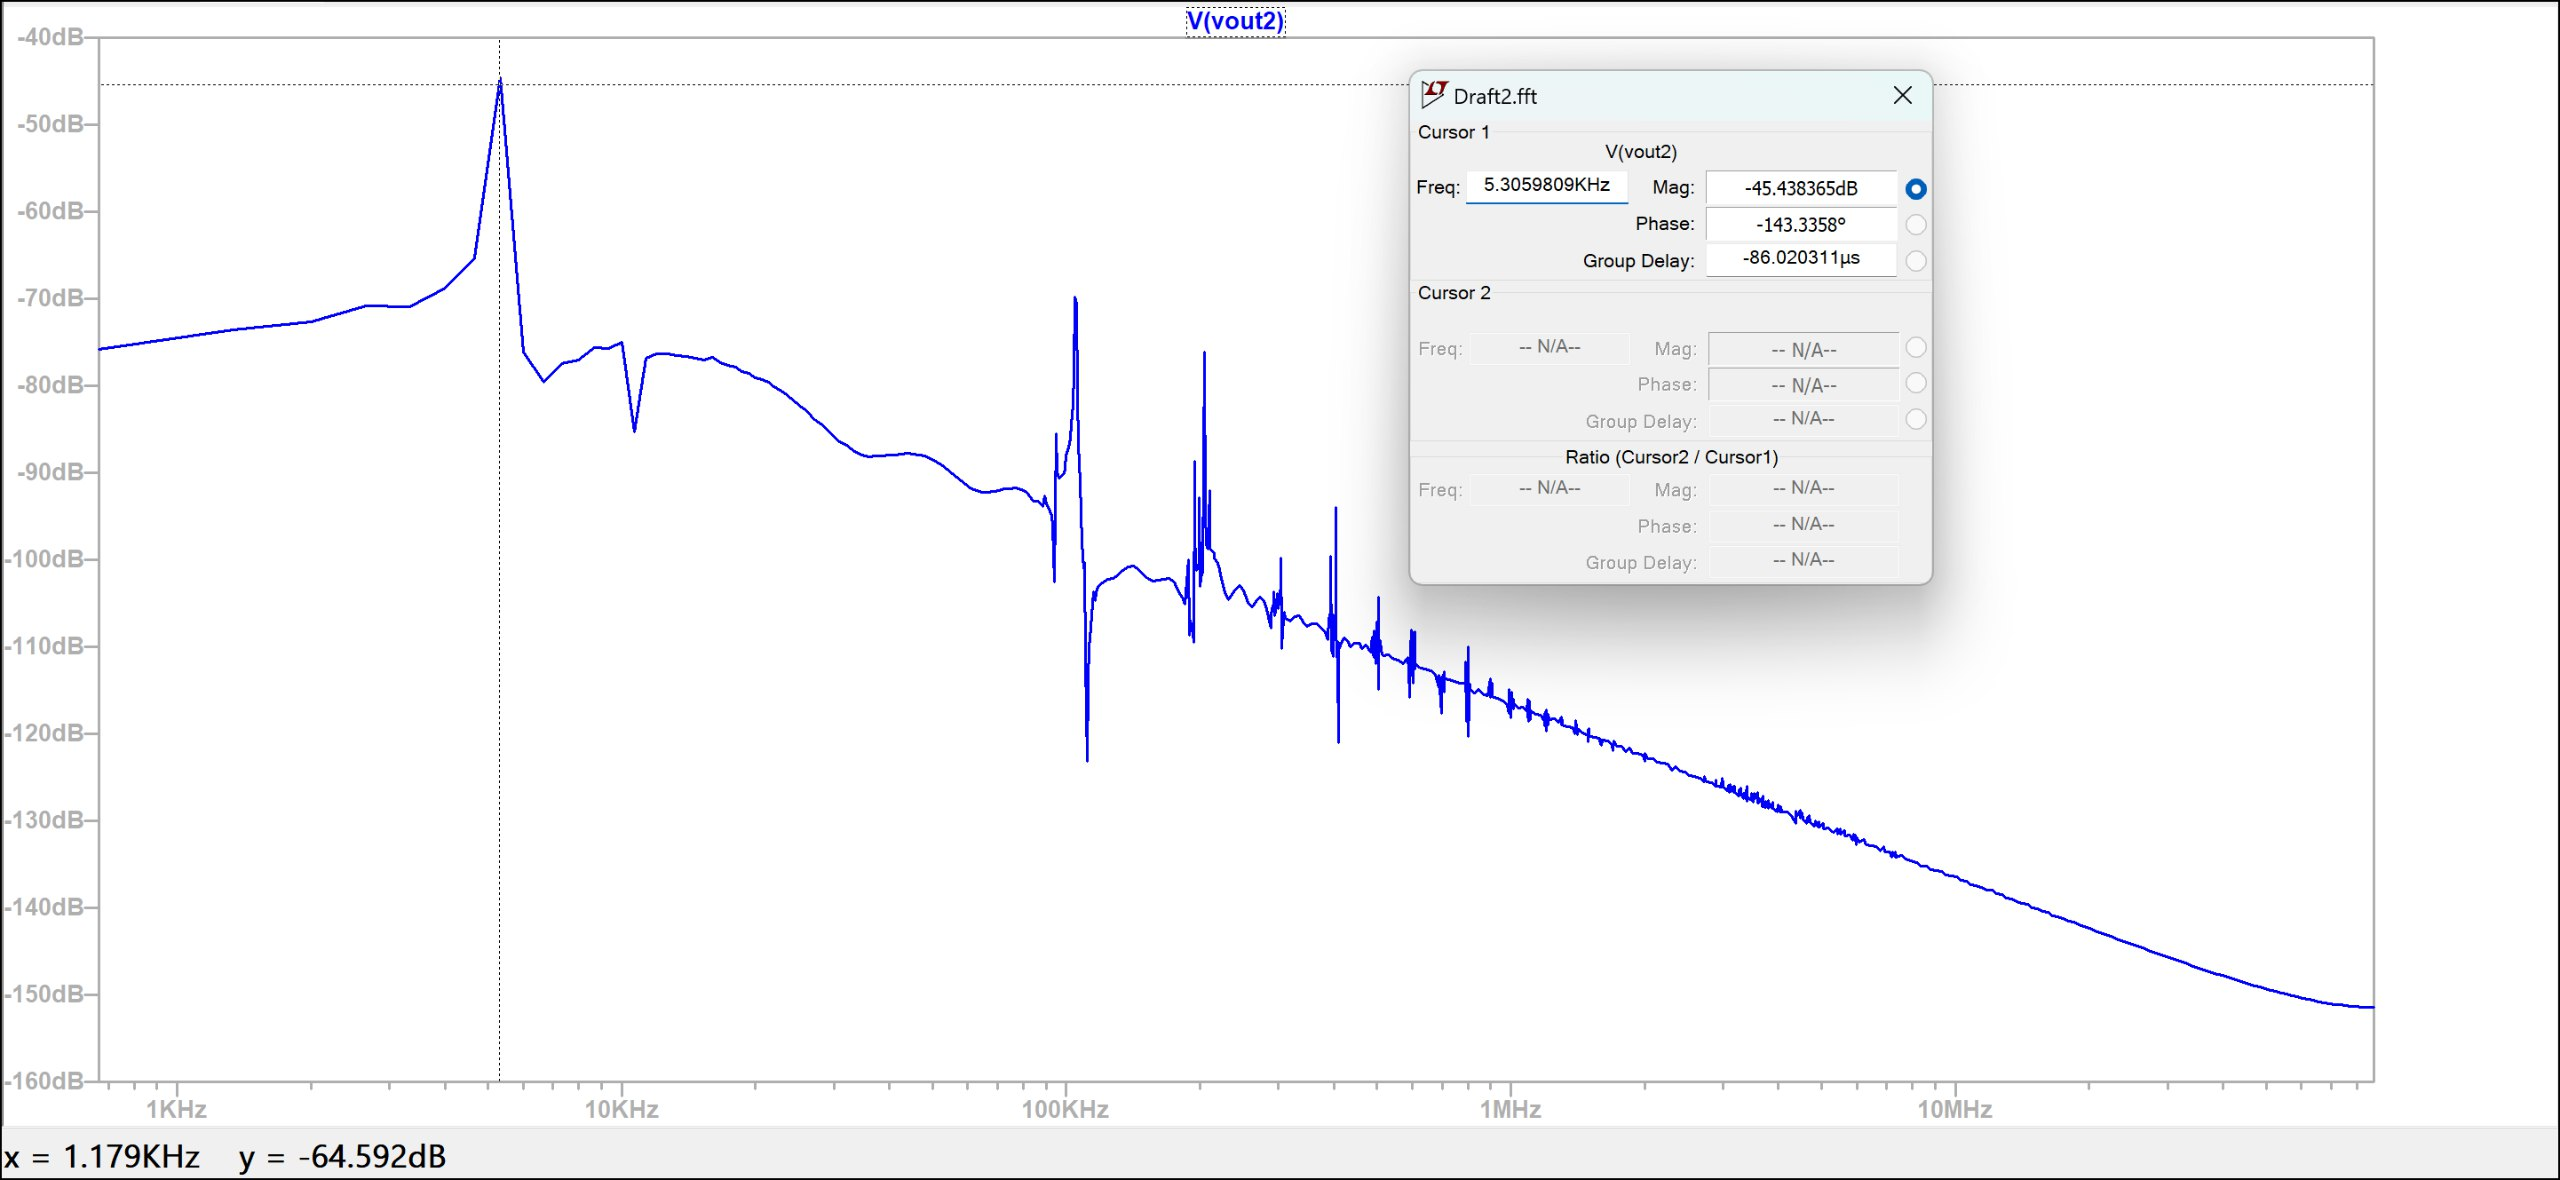
\includegraphics[scale=0.1]{final_fft2.jpeg}
\caption{ FFT plot of in-phase output}
\end{figure}

\begin{figure}[H]
\centering
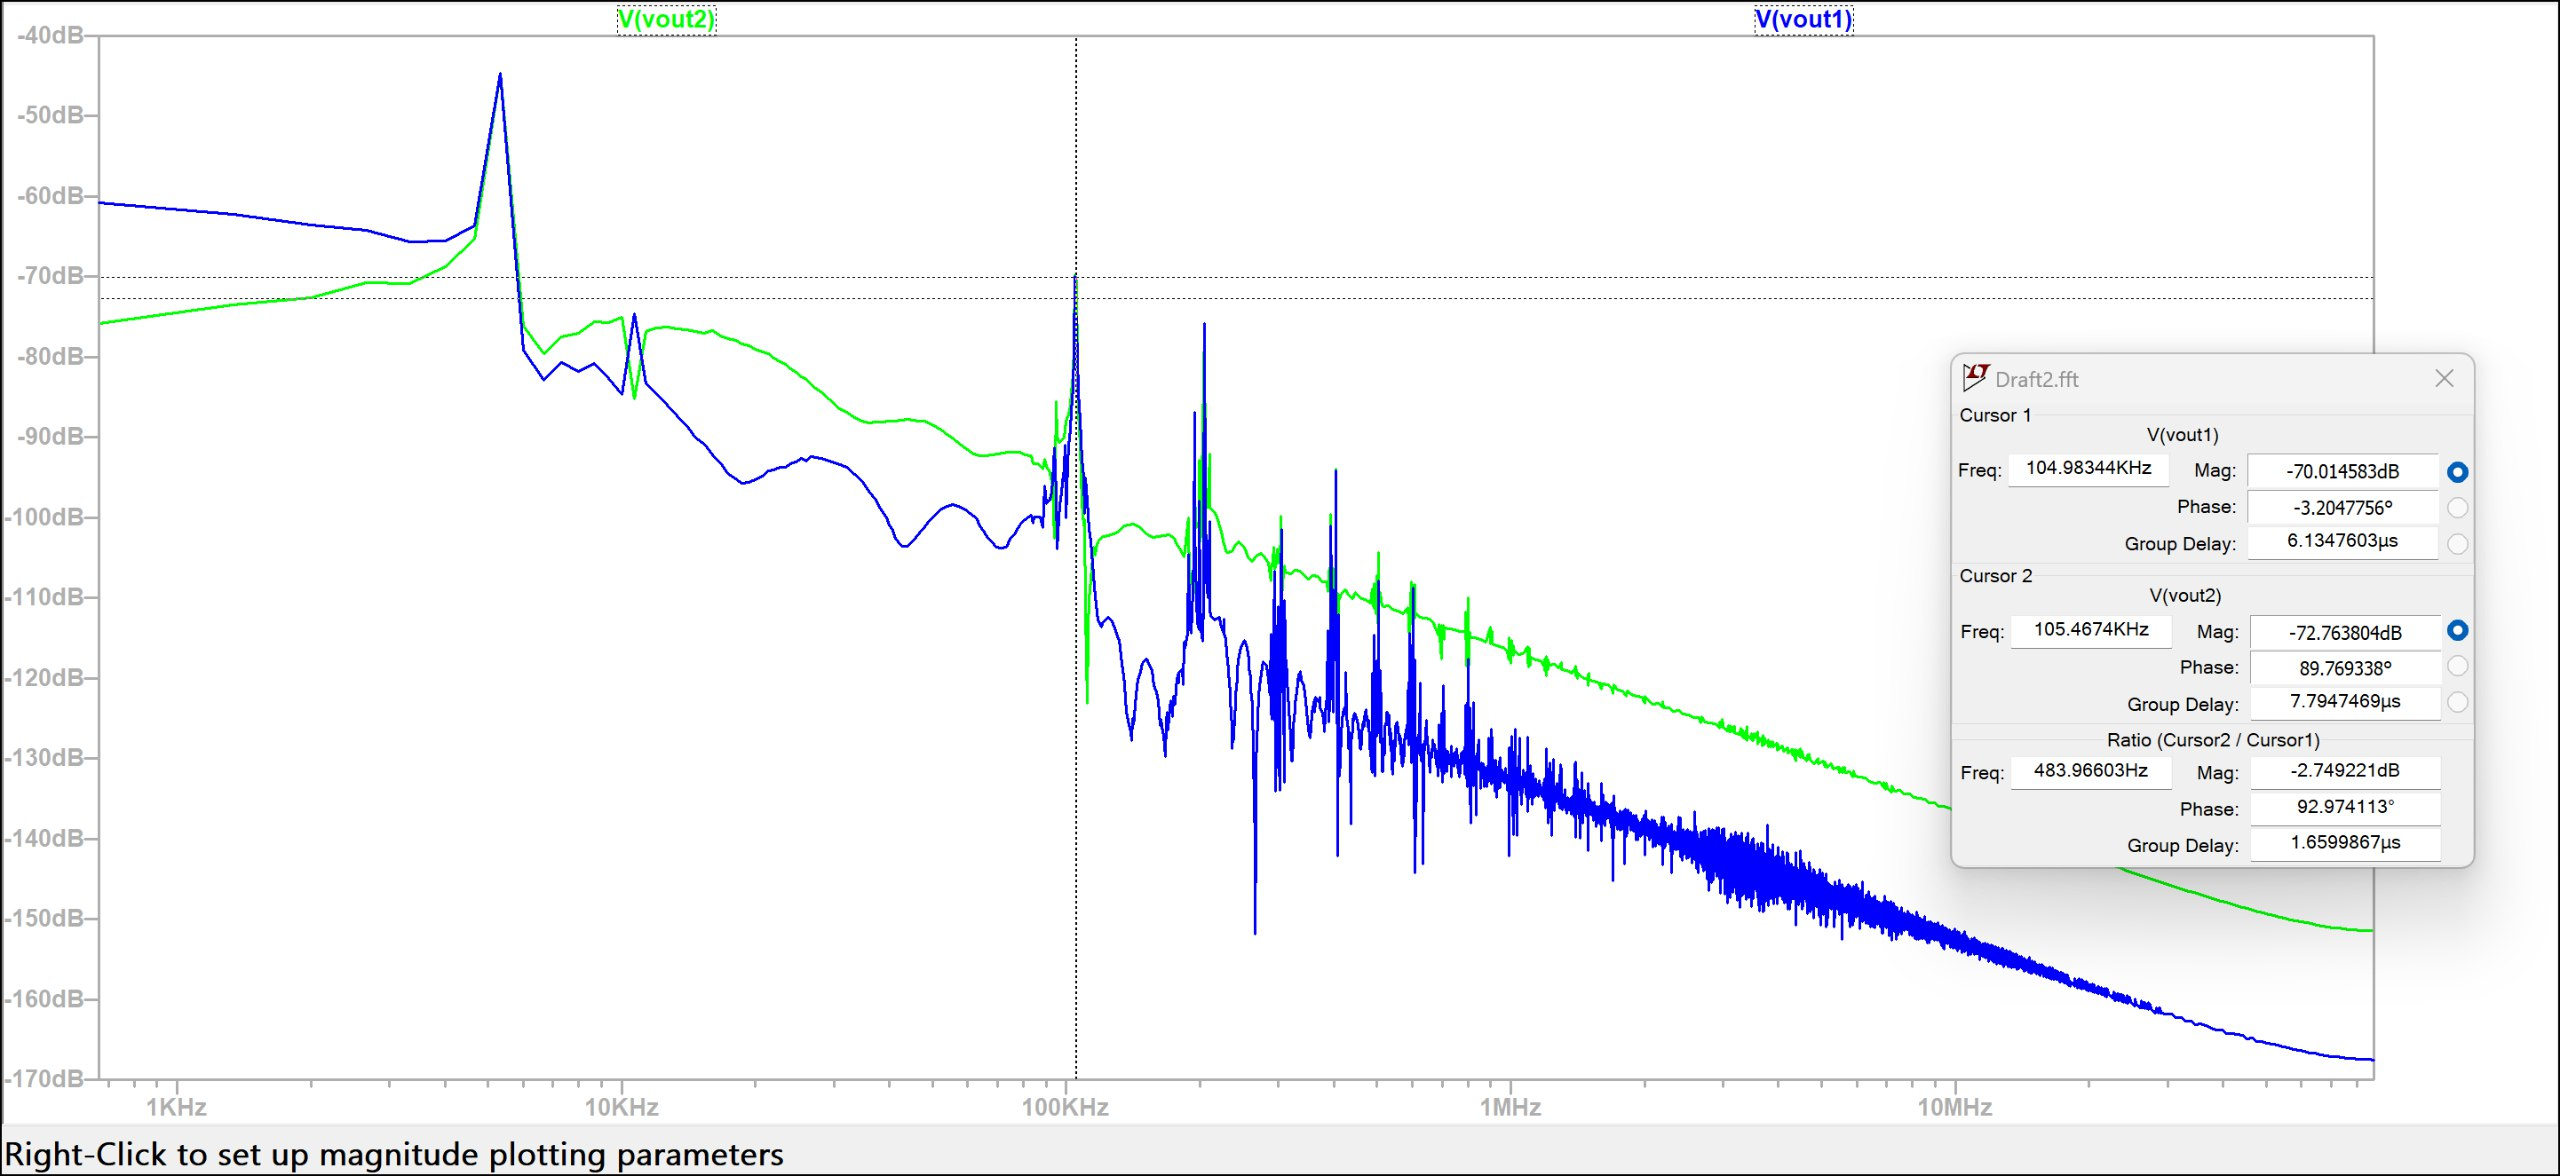
\includegraphics[scale=0.1]{final_fft.jpeg}
\caption{Combined FFT of both components, shows $92\degree$ phase difference}
\end{figure}

\section{ACKNOWLEDGMENT}
The authors would like to express their sincere gratitude to Prof. Zia Abbas for his exceptional teaching and continuous guidance throughout the course. We are also thankful to the Teaching Assistants for their insightful explanations and logistical support, which greatly contributed to the progress of our project. And finally we extend our appreciation to International Institute of Information Technology, Hyderabad for providing the necessary facilities and equipment.

\bibliographystyle{IEEEtran}
\bibliography{references} 
\cite{abidi1995direct}
\cite{mancini2001opamp}

\end{document}
